\title{Umělá inteligence}

\section{Umělá inteligence(UI) - Definice, úzká UI obecná UI, superinteligence, strojové učení}
Umělá intelgince je výpočetní systém vykonávající činnost, kterou si spojujeme s lidskou inteligencí\\
Další definice:
\begin{itemize}
    \item počítačové systémy, které jsou schopné plnit úkoly, které obvykle vyžadují lidskou inteligenci, jako je rozhodování, detekce objektů, řešení složitých problémů
    \item vědní disciplína, zabývající se teoríí systémů zpracovávajících data a schopných se víceméně samostatně rozhodovat
    \item schopnosti počítače/algoritmu napodobovat/realizovat některé funkce lidského mozku
\end{itemize}
\subsection{Úzká umělá inteligence}
stupeň UI zahrnující stroje, které mohou provádět pouze úzce definovaou sadu konkrétních úkolů\\
jediná forma, které lidstvo doposud dosáhlo\\
aplikace na rutinních pracích - rozpoznávání řeči, obrazu, počítačové vidění, inteligentní budovy, hra šachů, návrh nákupu, počasí\\
UI je vznešený název pro sofistikované SW řešení, vkládáme důvěru do autora, že nic neopomenul\\
\begin{figure}[H]
    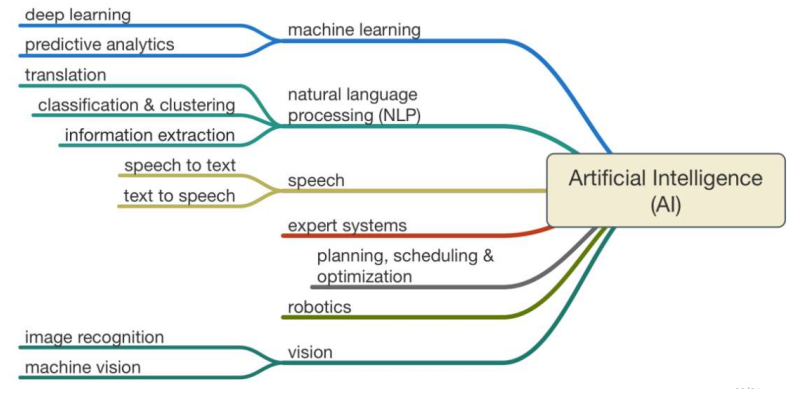
\includegraphics[scale = 1]{images/uzkeAI.png}
\end{figure}
\subsection{Obecná UI}
Umělá inteligence na úrovni člověka\\
umí se rozhodovat, komunikovat, samostatně se učit\\
zatím není vyvinuta\\
Tuninguv test - nemožnost rozeznat člověka od stroje\\

\subsection*{Superinteligence}
má vyšší inteligenci než člověk\\
uvědomuje si, že ji ovládají a omezují intelektuálně podřadní lidé\\



\subsection{Strojové učení(machine learning)}
Podoblast umělé inteligence, zabývající se algoritmy a technikami, které počítačovému systému umožňují se učit.\\
Učení v tomto případě znamená využívání dat pro zlepšení efektivity plnění úkolů určitého druhu.\\
Má 2 základní části:
\begin{itemize}
    \item Deep learning
    \item Predictive analytics
\end{itemize}

Základní přístupy ke strojovému učení:
\begin{itemize}
    \item Učení s učitelem (Supervised learning)
    \item Učení bez učitele (Unseupervised learning)
    \item Kombinace učení s učitelem a bez učitele (Semi-supervised learning)
    \item Zpětnovazební učení, též učení posilování (reinforced learning)
\end{itemize}

\subsubsection{Deep learning}
Druh algoritmů storjového učení, který používá vícevrstvých neuronových sítí pro extrakci rysů ze surových dat, v čím pokročilejší vrstvě jsme tím vyšší úroveň rysy mají.\\
Jako příklad mějme ve zpracování obrazu, kde v nižší vrstvy identifují hrany v obraze a vyšší vrstvy již identifikují věci relevatní pro člověka, například písmena nebo číslice.\\
Většina modelů hlubokého učení je založená na umělých neuronových sítích(většinou konvolučních).\\
Mohou však také být založeny na statisticky založených hlubokých generativních modelech (deep generative models), tyto modely používají učení bez učitele a jsou založeny na statistickém rozložení dat v trénovací množině a dělat rozhodnutí založená na podobnosti charakteristiky předložených dat. Příklady těchto modelů jsou Deep belief network (DBN) a Boltzamannův stroj.\\
\subsubsection{Predictive analysis}
Proces využívání statistických modelů kde studiu dat a identifikaci vzorců, kterými se mohou předpovídat budoucí události či chování. Využívá se například pro predikci prodejů, finančního chování, doporučování reklam na základě historie prohlížení uživatele, atd.\\
\subsubsection{Učení s učitelem}
\label{typ_uceni}
Data jsou rozdělena na trénovací, validační a testovací\\
Učení probíhá tak, že systému předkládáme trénovací vzory a zároveň požadované výstupy, na základě kterých se mění váhy.\\
Trénování modelu je hledání matematické funkce, která mapuje předložené vstupy na žádané výstupy. Cílem je minimalizace chyby mezi žádanými a spočítanými výstupy.\\
\newpage
\begin{figure}[h!]
    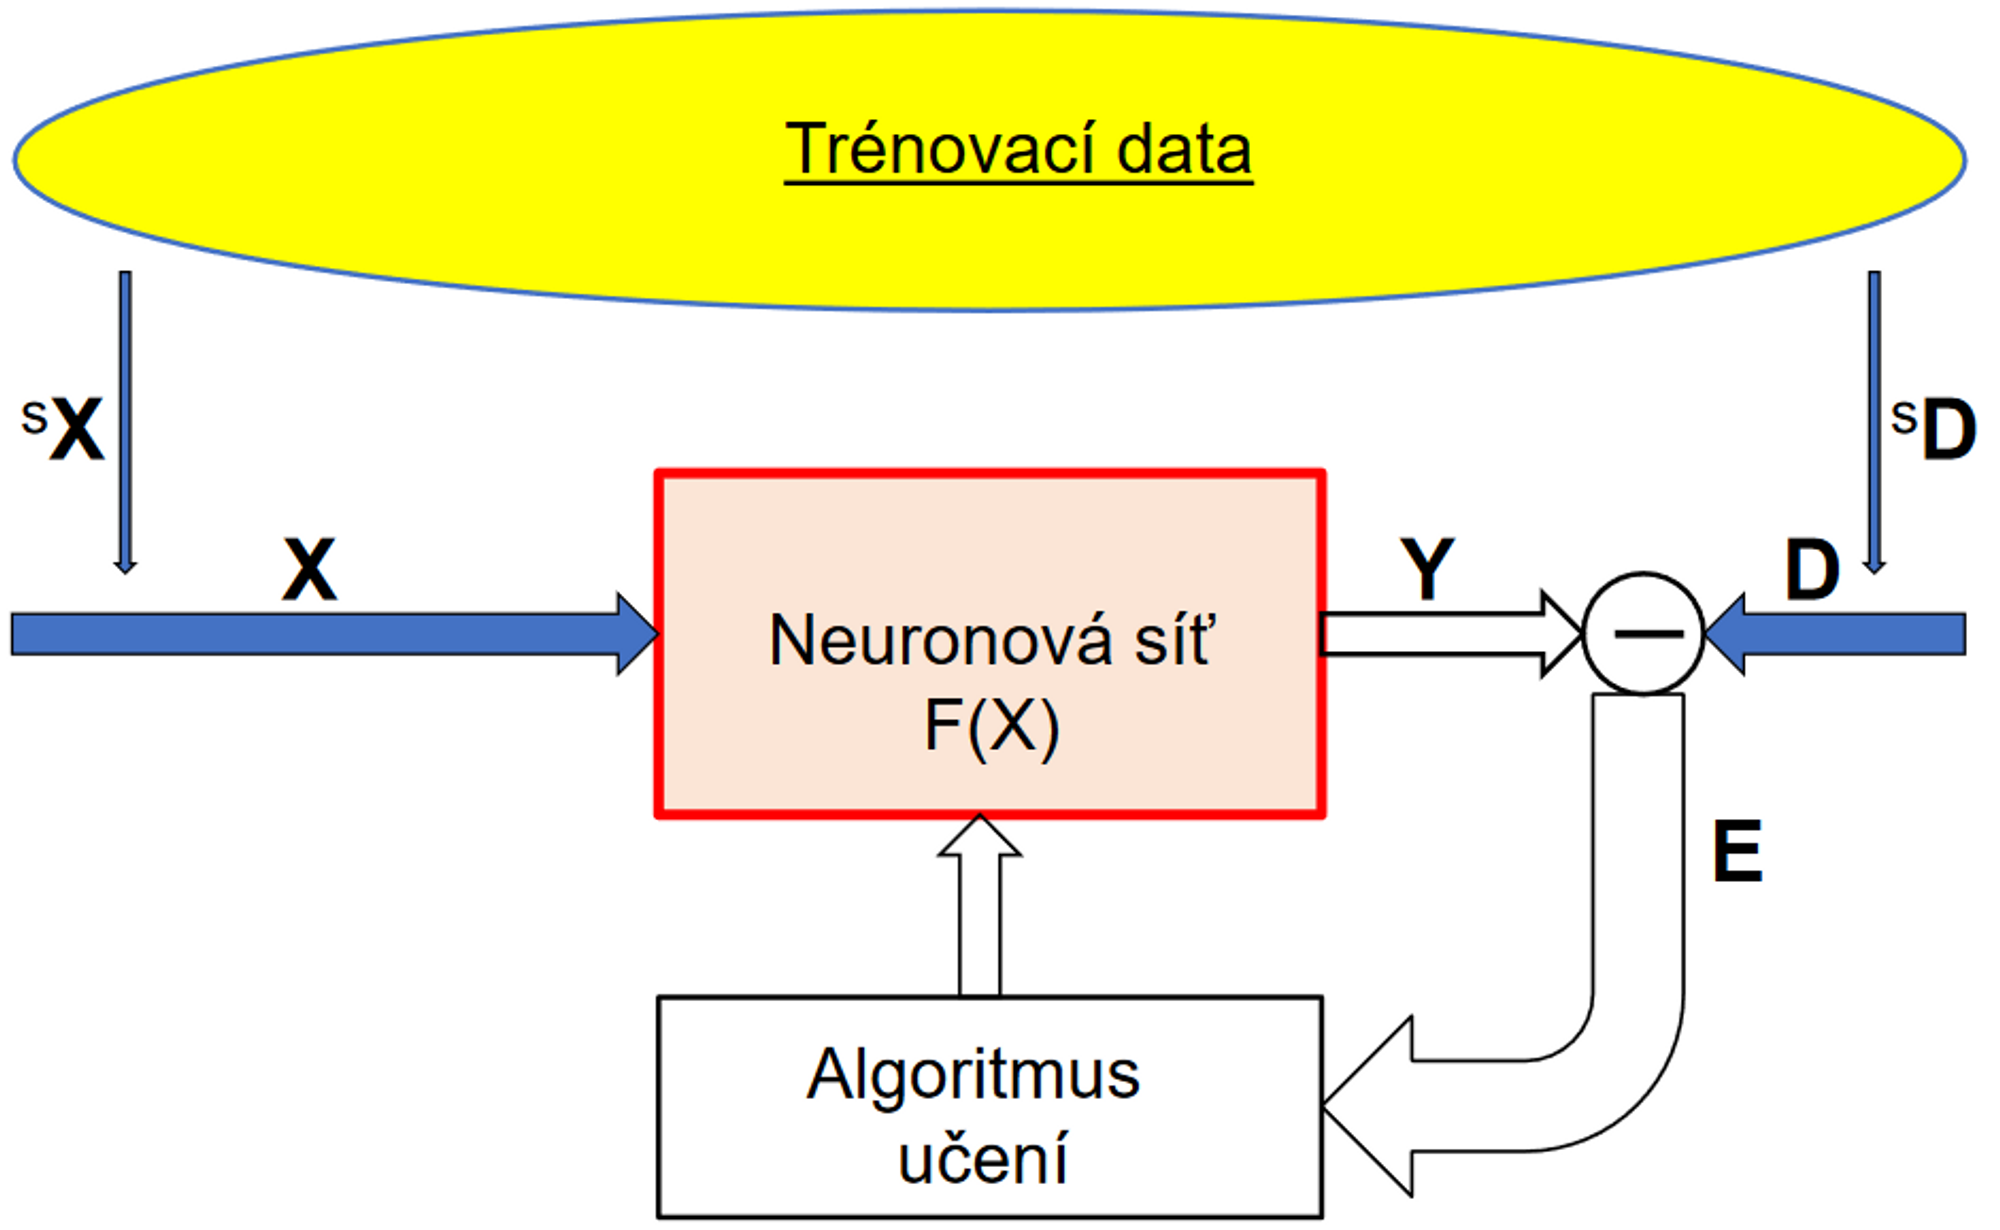
\includegraphics[scale = 0.3]{images/sUcitelem.png}
\end{figure}

\subsubsection{Učení bez učitele}
Data jsou pouze jednoho typu a to trénovací\\
Učení probíhá tak, že jsou systému předloženy sady vstupů(bez správných výsledků, protože je neznáme) a na základě vstupů se mění váhy.\\

Úkolem je identifikovat podobné shluky, vzory či anomálie v datech. Toto se často provádí buď pomocí shlukování(clustering) nebo redukováním dimenzionality(dimensionality reduction). Při shlukování se podobné instance řadí do shluků na základě jejich podobnosti. Příklady algoritmů shlukování jsou K-means, hierarchické shlukování nebo DBSCAN.

\begin{figure}[h!]
    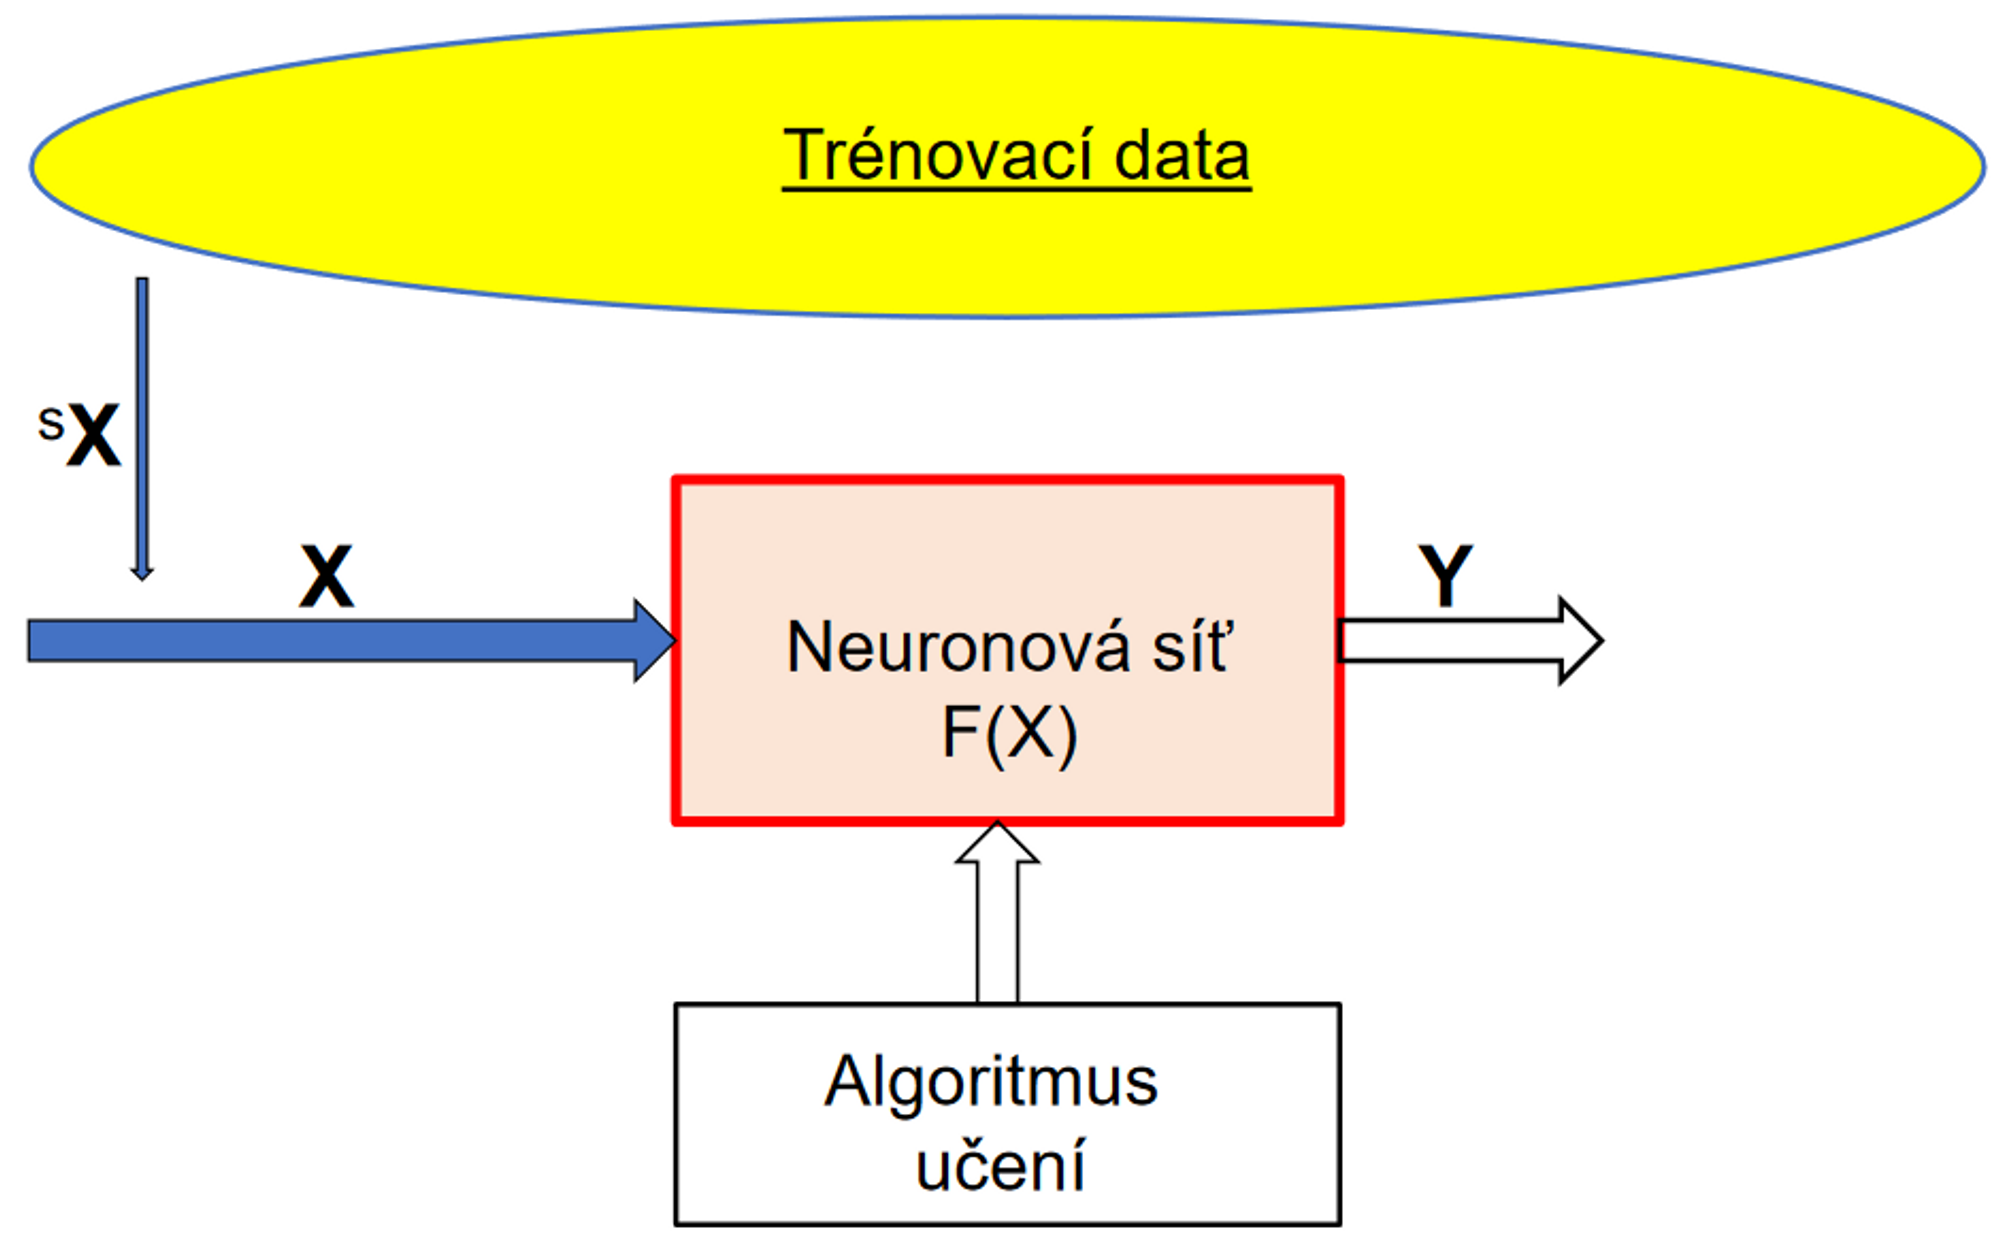
\includegraphics[scale = 0.3]{images/bezUcitele.png}
\end{figure}

\subsubsection{Kombinace s učitelem a bez učitele}
Kombinuje přístupy dvou předchozích přístupů, kde máme jak data označkovaná jako v učení s učitelem, tak neoznačkovaná jako je tomu v učení bez učitele.\\

Cílem semi-supervised learningu je využít označkovaných dat pro trénování modelu a neoznačkovaných dat pro zlepšení výkonu modelu. Využití neoznačkovaných dat zlepšuje představu modelu o celké struktuře dat a vede k lepší generalizaci.\\

Obvykle je více neoznačkovaných jak označkovaných dat.\\

Učení probíhá tak, že se prvně používá metod supervised learnigu a poté se model rozšíří tak aby pracoval s neoznačkovanými daty, kde se využívá například generativních modelů, založených na statistickém rozložení dat, či využití clusteringu pro získání struktury neoznačkovaných dat.\\

Hlavní výhodou je využití nezonačkovaných dat, která jsou dostupnější než data označkovaná, tím snižujeme časový náklad na nutnost označkovat všechny data.\\

\subsubsection{Zpětnovazební učení}
Technika učení zaměřená na trénování například robota na základě interakce s okolím. V tomto přístupu není přede označkovaná trénovací množina nebo příklady správných výsledků, ale funguje na základě zpětné vazby v podobě odměn či trestů získaných při provádění různých akcí v prostředí.\\
Během učení agent zkouší různé strategie a akce a snaží se najít takovou, která maximalizuje příjem v dlouhodém horizontu. Pro toto se využívají například metody Q-learning či metoda Monte Carlo.\\
Q-learning se snaží určit optimální hodnotovou funkci, která se každému stavu a akci snaží přiřadit očekávaný kumulativní příjem, optimalizací této funkce se vybírají akce v prostředí pro co největší příjem.\\
Monte Carlo odhaduje hodnotovou funkci na základě průměru náhodně prováděných akcí a jejich odměn.\\

\subsection{Základní druhy úloh}
\begin{itemize}
    \item Klasifikace vstupních dat do tříd
    \item Odhadování výstupní hodnoty podle vstupu
    \item Zařazování objektů do skupin podle podobných vlastností - učení bez učitele
\end{itemize}

\section{Umělé neuronové sítě - paradigmata, perceptron, algoritmus Backpropagation, Kohonenova samoorganizační mapa, konvoluční neuronová síť}
\subsection{Paradigmata}
použité modely neuronů\\
topologie\\
způsob učení\\
způsob vybavování\\

\subsubsection{Neuron}
\begin{figure}[H]
    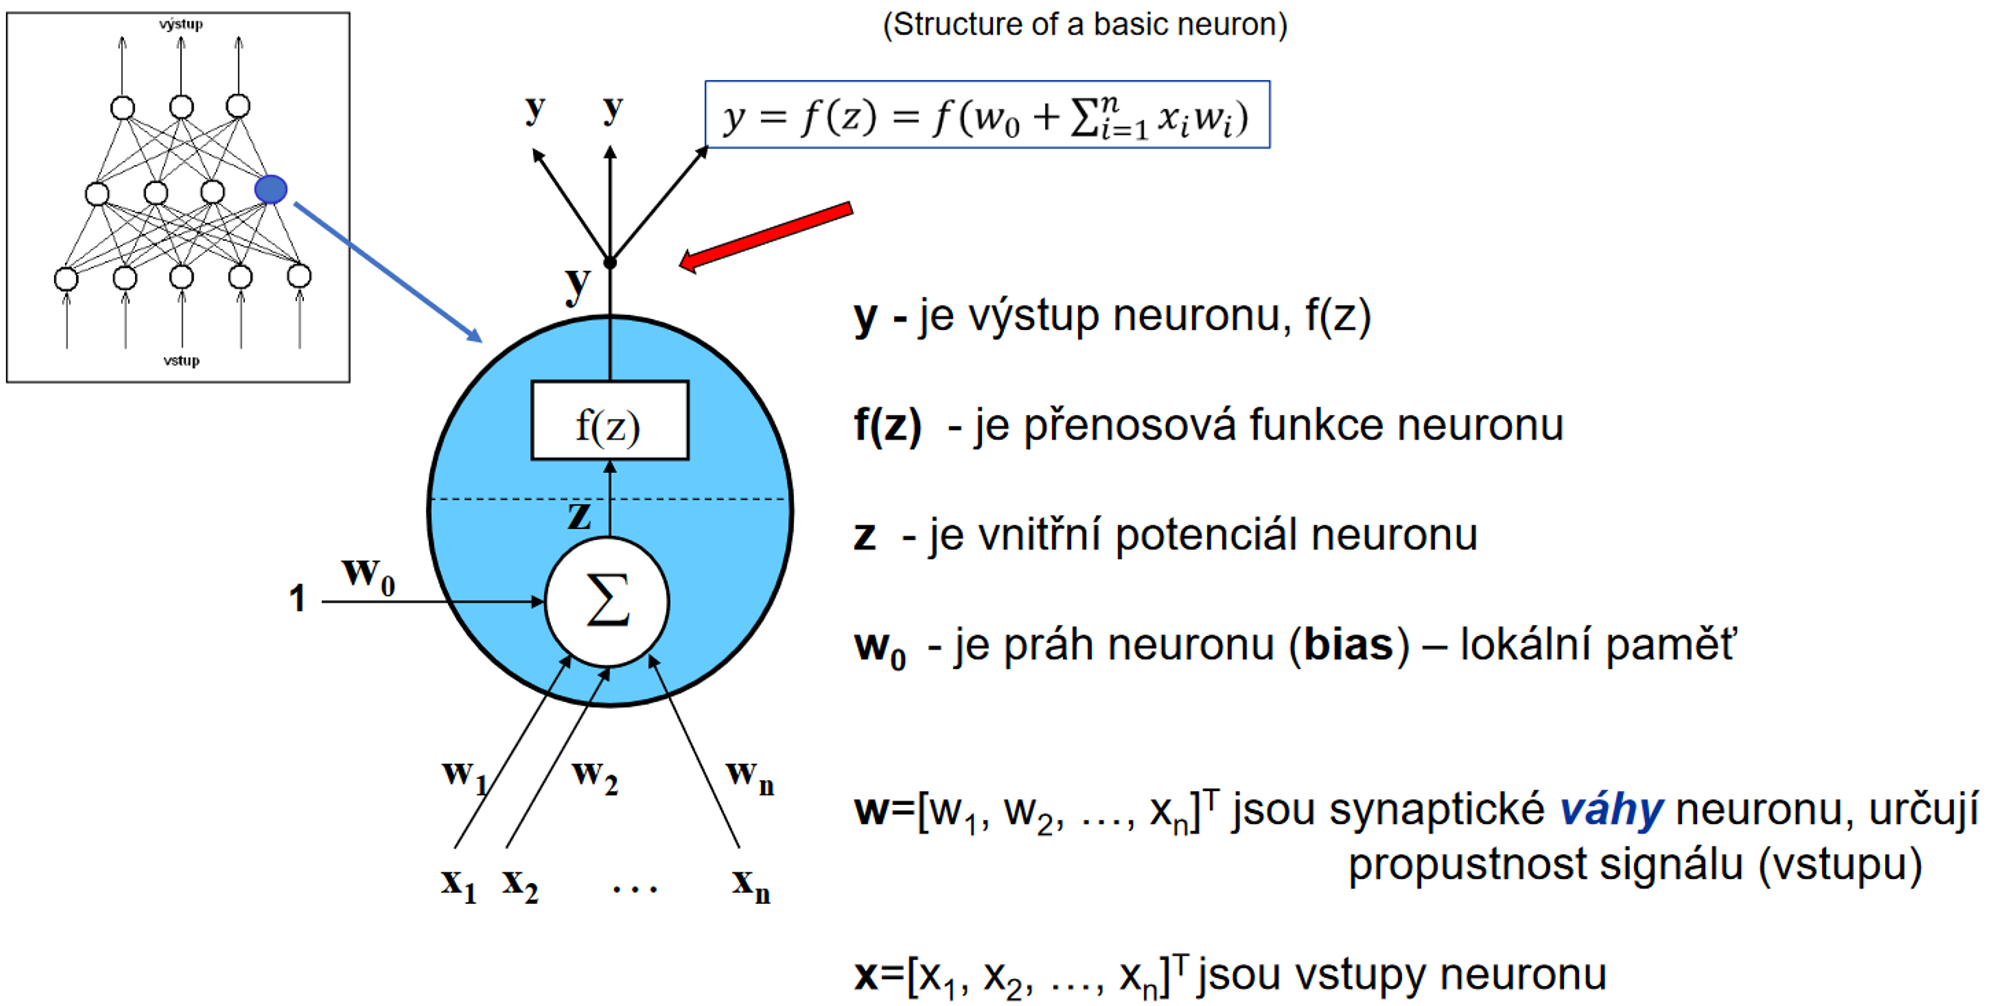
\includegraphics[scale = 0.5]{images/neuron.png}
\end{figure}
vnitřní potenciál neuronu je lineární, nebo radiální
\begin{itemize}
    \item lineární: $z = w_0 + \sum^n_{i=1}x_iw_i$
    \item radiální: $z = w_0 + \sqrt{\sum^n_{i=1}(x_i-w_i)^2}$
\end{itemize}

\subsubsection{Topologie}
Orientovaný graf
\begin{itemize}
    \item neurony tvoří uzly grafu
    \item hrany grafu se nazývají spoje
    \item každý spoj má váhu
    \item každý neuron má libovolný počet vstupů a výstupů(stejných)
    \item každý neuron má bias, vnitřní potencíál a přenosovou funkci
\end{itemize}
struktura je Přímovazební nebo zpětnovazební:
\begin{figure}[H]
    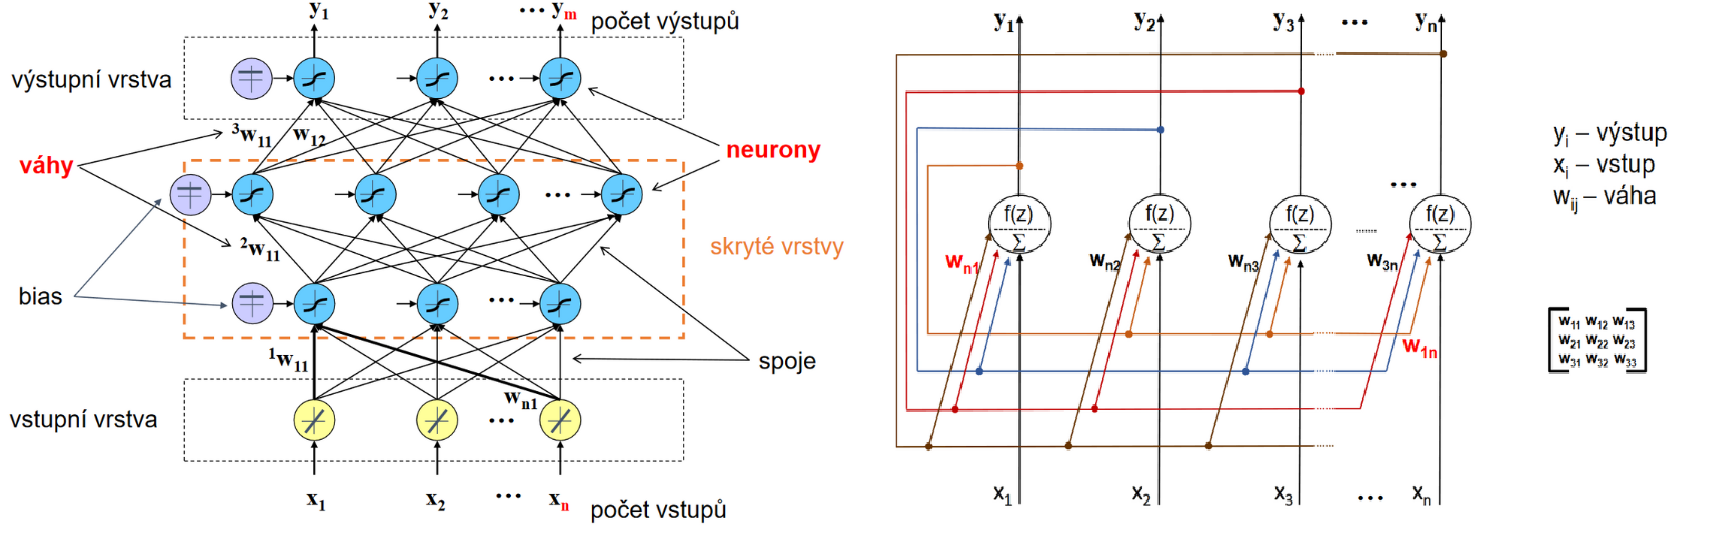
\includegraphics[scale = 0.5]{images/struktury.png}
\end{figure}

\subsubsection{Učení popsáno v předchozí otázce viz \ref{typ_uceni}}

\subsubsection{Vybavování}
aktivní režim\\
vlastní výpočet funkce naučené neuronové sítě na daný vstup\\
jsou dva typy:
\begin{itemize}
    \item jednorázový - přímovazební, odezva probíhá v jedné iteraci
    \item iterační proces - zpětnovazební, odezva probíhá iterativně
\end{itemize}

\subsubsection{Aplikace}
regrese - predikce spojité proměnné na základě vstupu\\
klasifikace - zařazení do tříd(detekce spamu, jestli poslat pacienta na dané vyšetření)\\
časové řady - jak regrese tak klasifikace\\
shluková analýza - učení

\subsection{Perceptron}
Charakteristika:
\begin{itemize}
    \item neuron - nespojitá přenosová funkce
    \item topologie - jednovrstvá přímovazební
    \item učení - iterativní, s učitelem
    \item tréninková množina - \textbf{lineárně separabilní}
    \item vybavování - jednorázový proces
    \item aplikace - lineárně separabilní klasifikátor
\end{itemize}
\subsubsection{Neuron}
\begin{figure}[H]
    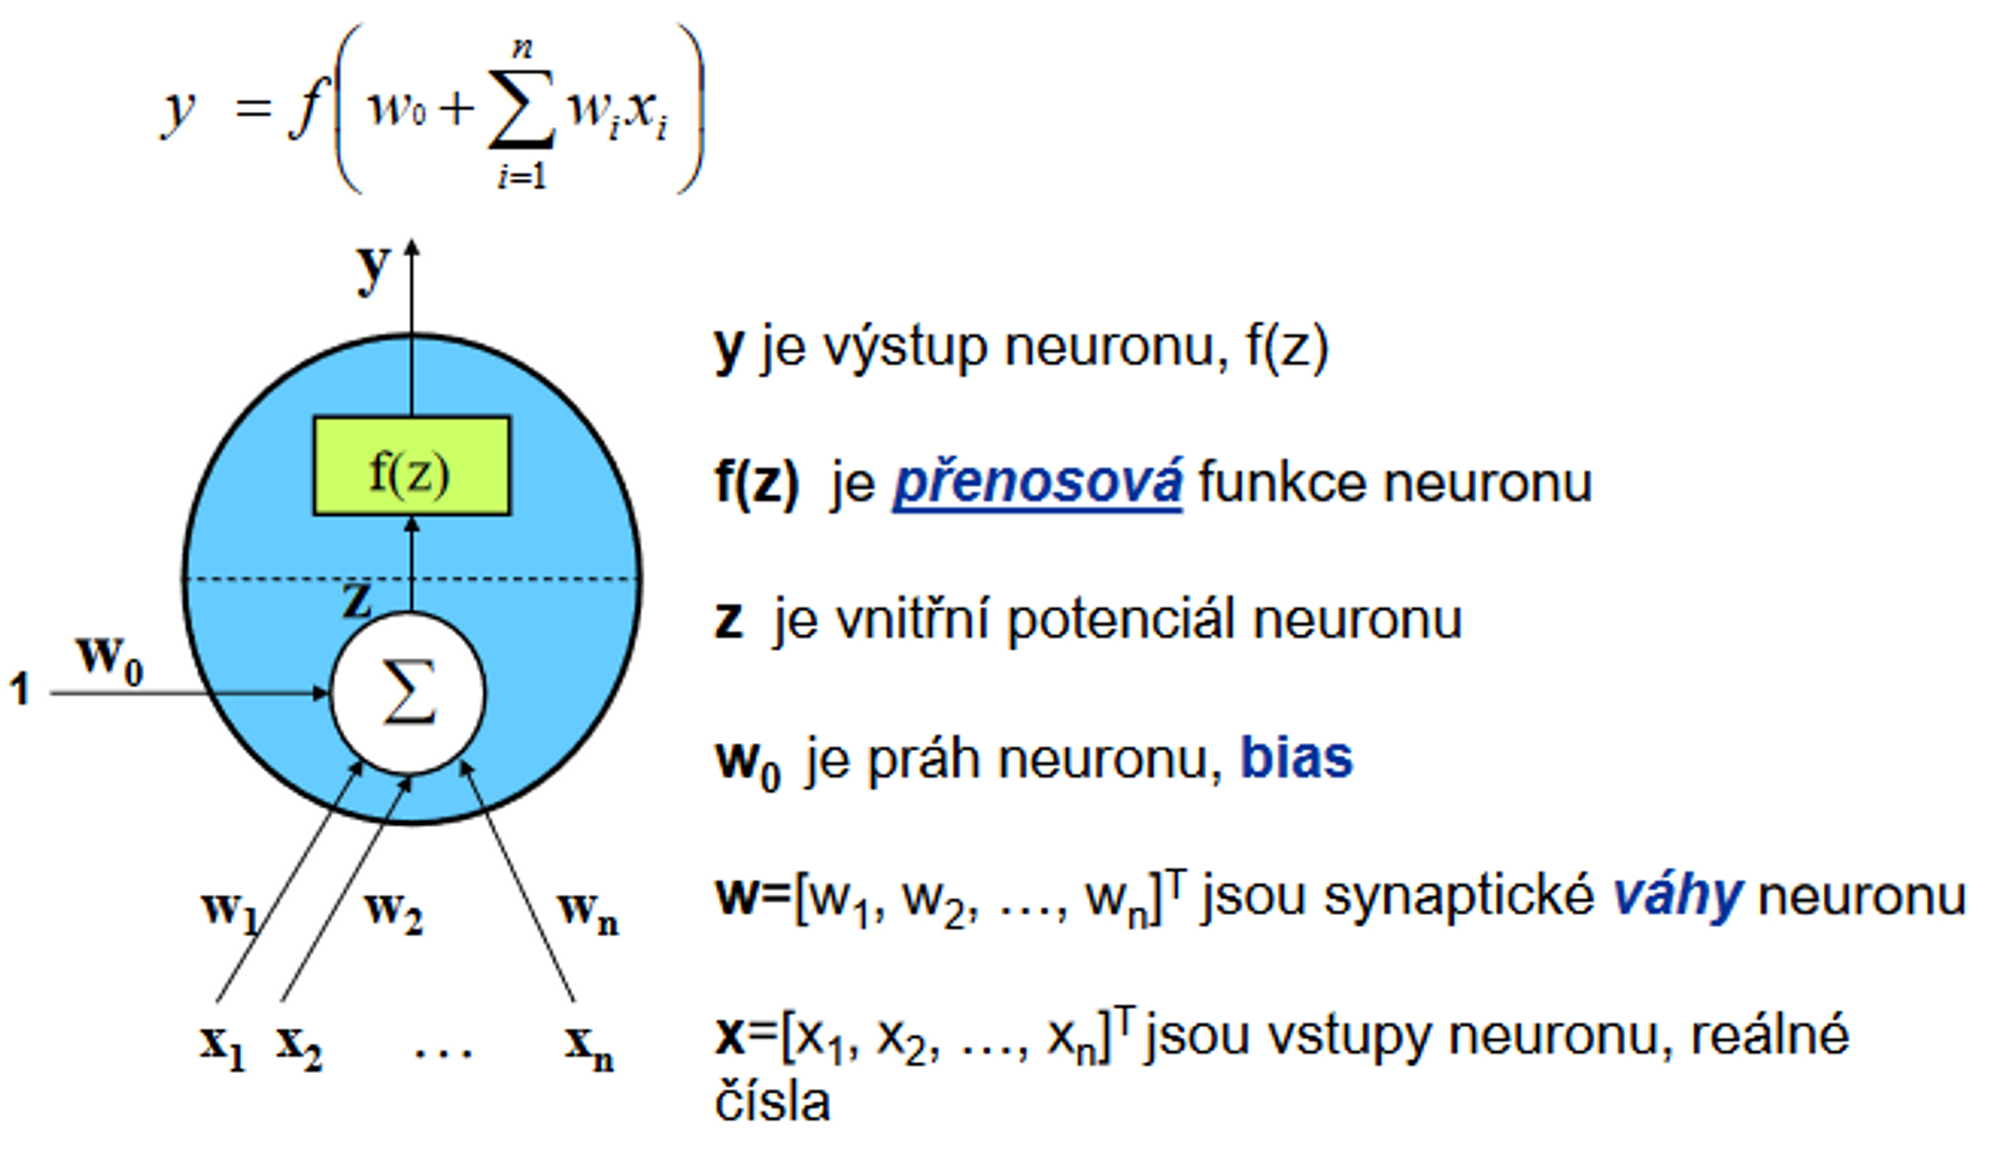
\includegraphics[scale = 0.2]{images/perceptron_neuron.png}
\end{figure}
\newpage
Přenosová funkce bez prahu:
\begin{figure}[H]
    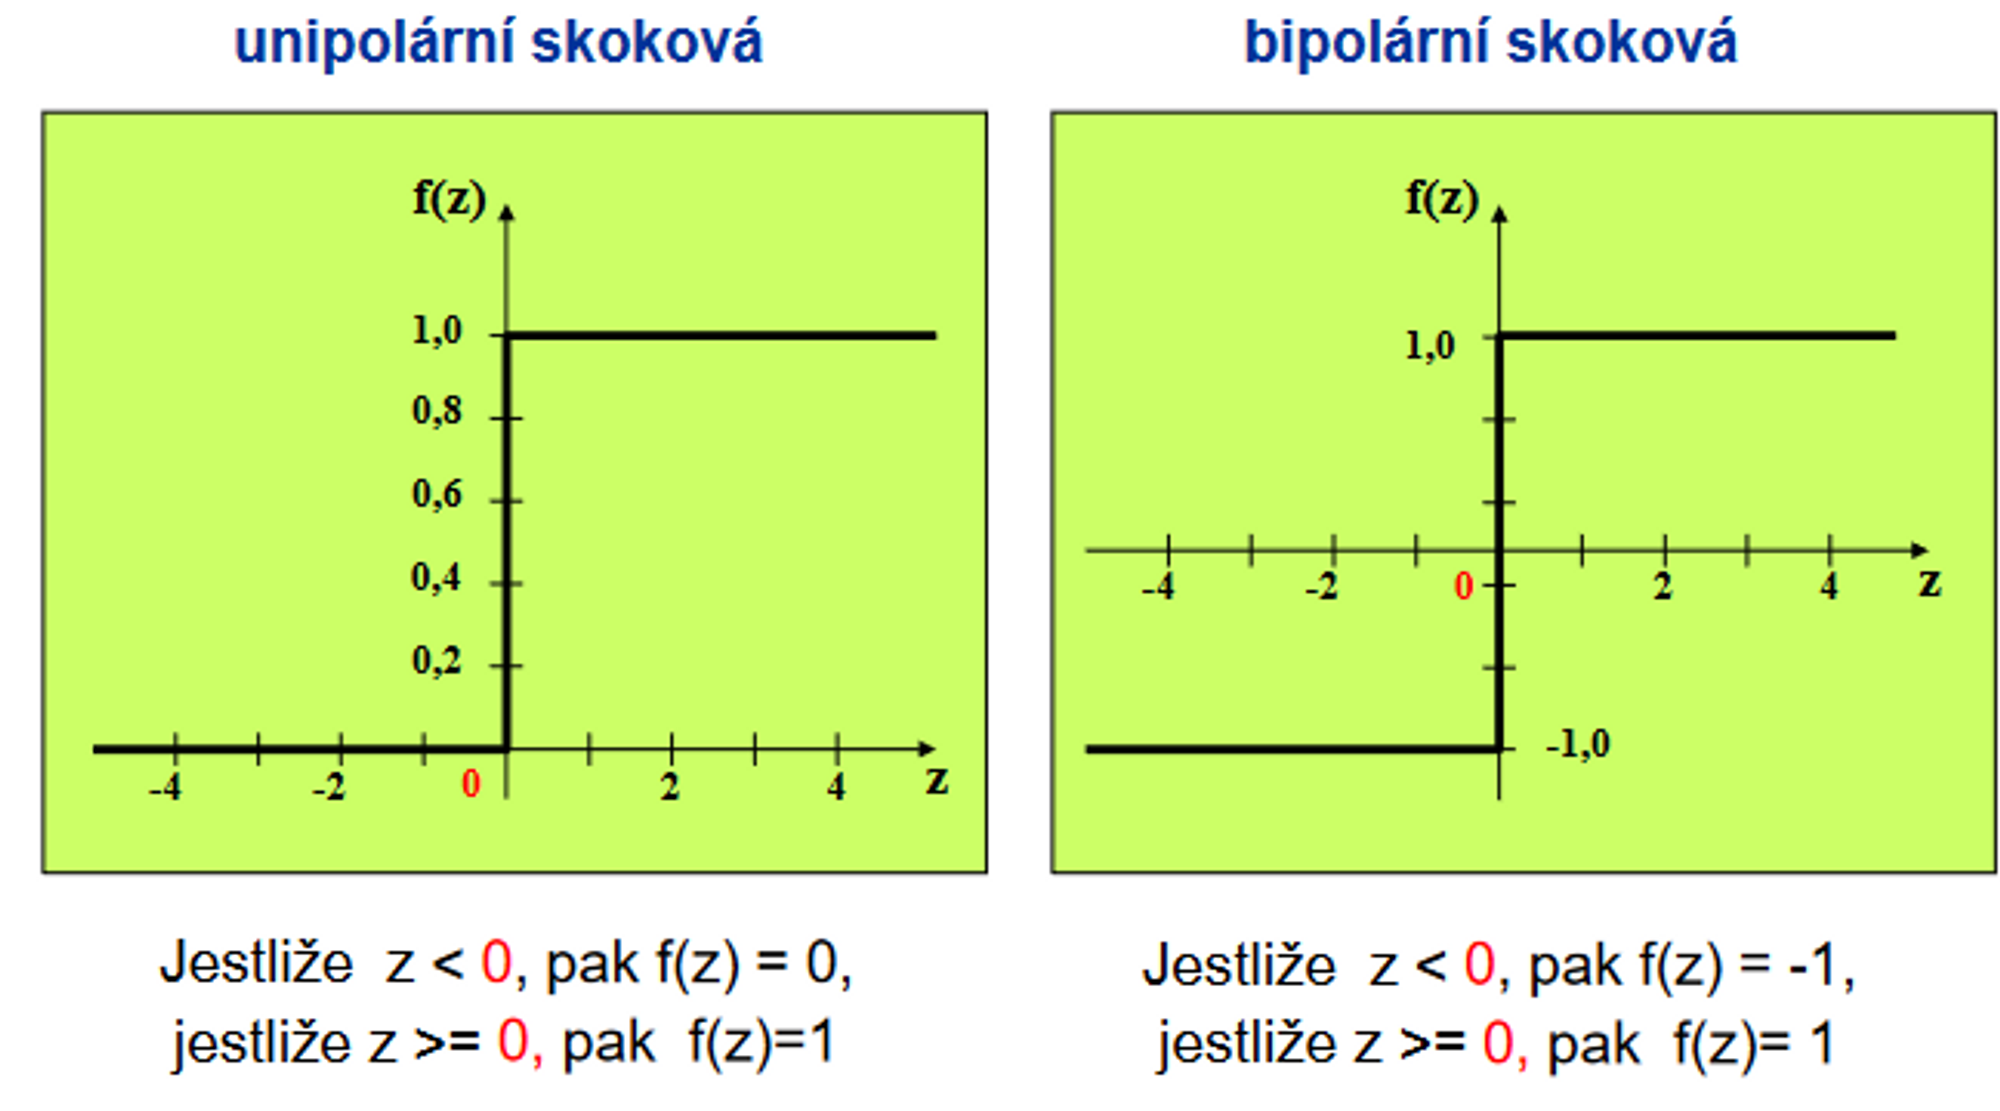
\includegraphics[scale = 0.2]{images/perceptron_prenos.png}
\end{figure}
Přenosová funkce s prahem
\begin{figure}[H]
    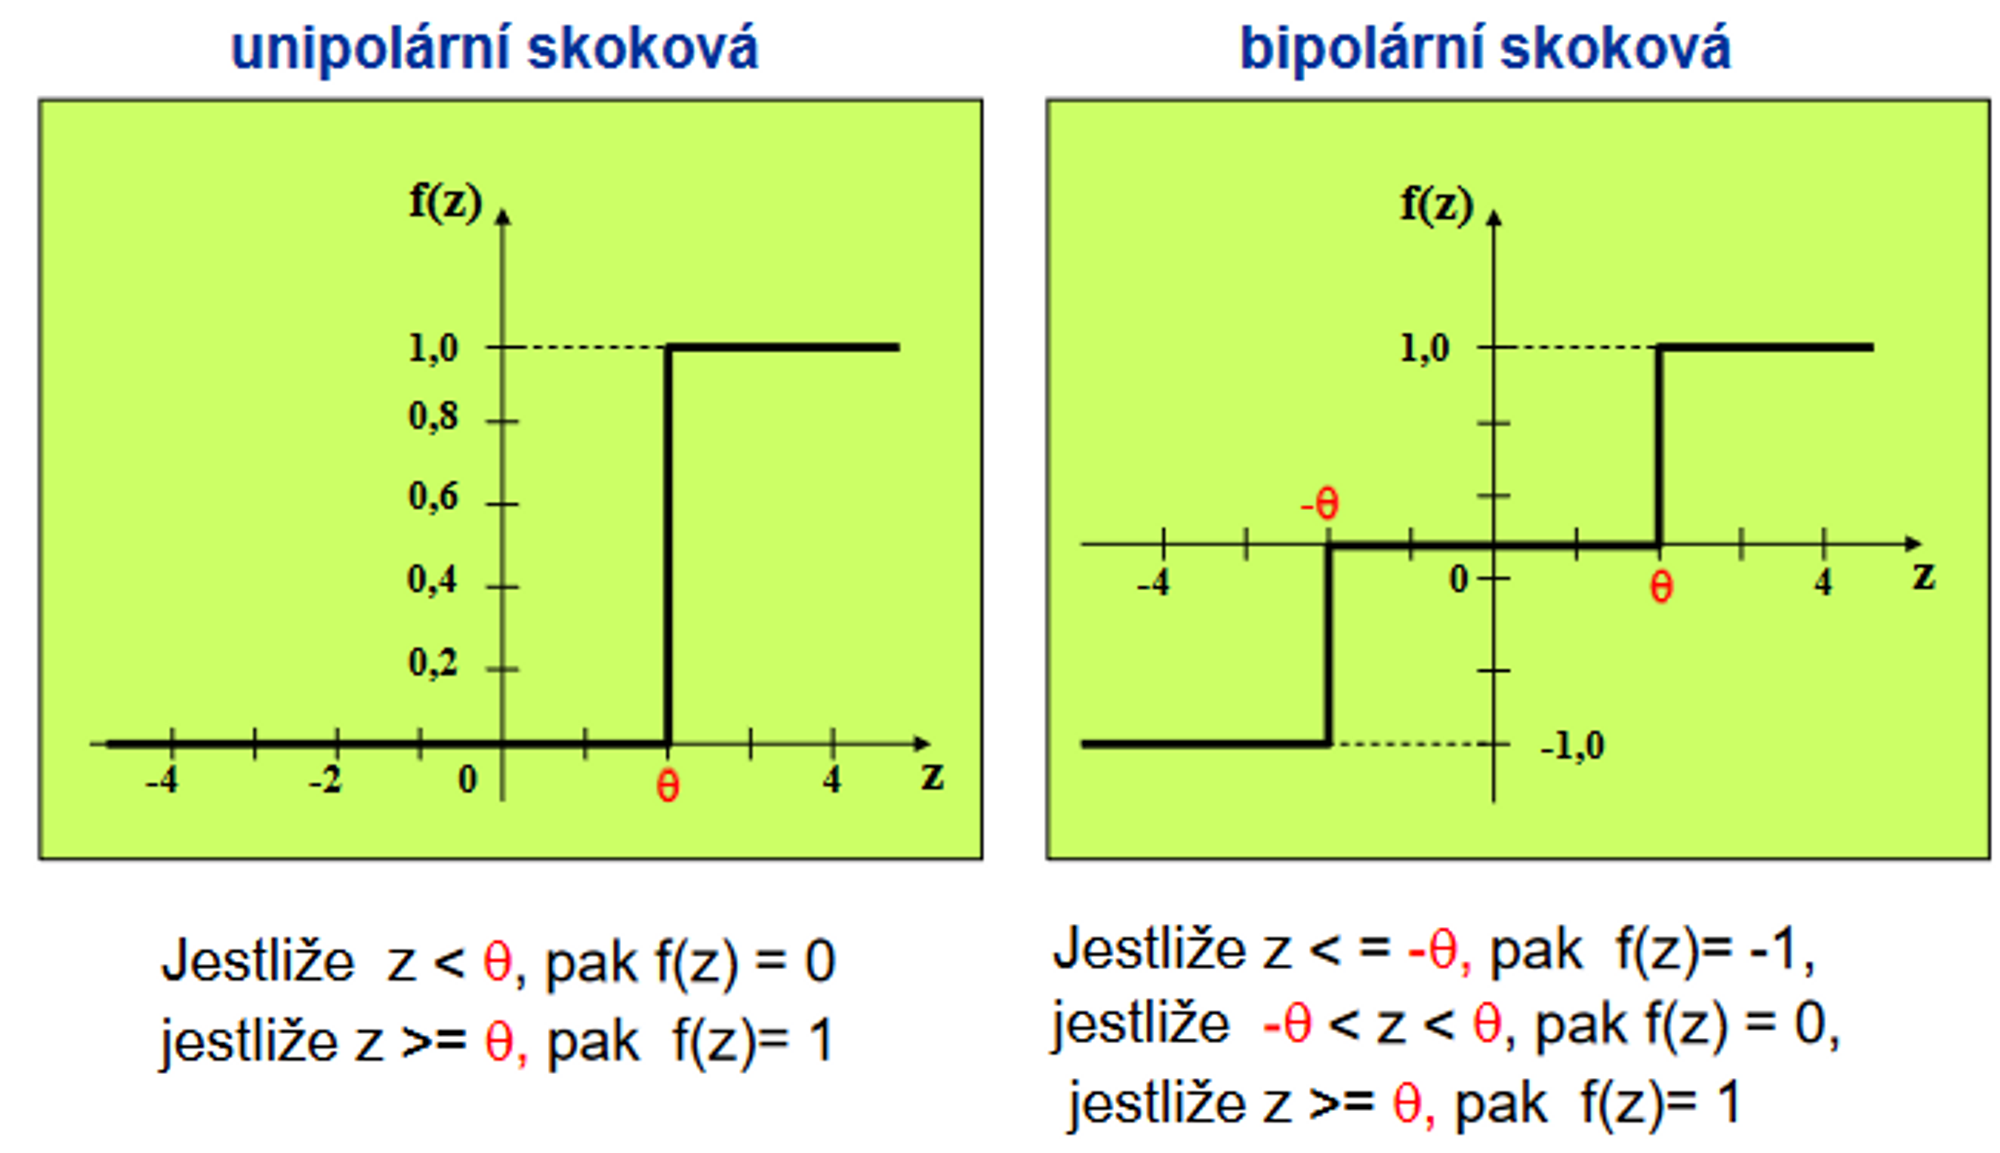
\includegraphics[scale = 0.2]{images/perceptron_prenos_s_prahem.png}
\end{figure}

\subsubsection{Topologie}
jeden nebo více perceptronů
\subsubsection{Učení}
když je v n-rozměrném rostoru lineárně separabilní třída objektů, v konečném počtu kroků učení lze najít vektor vah perceptronu, který je oddělí\\
Kroky učení:
\begin{enumerate}
    \item Start, inicializace(nastavení vah a určení přenosové funkce)
    \item předložení tréninkového vzoru
    \item výpočet výstupu sítě
    \item učení - adaptace vah
    \item test na shodu
    \item test na ukončení - jestli jsou všechny klasifikace správně
\end{enumerate}
Nastavení vah je na malá náhodná čísla\\
Adaptace vah probíhá třemi různými způsoby:\\
A):
\begin{figure}[H]
    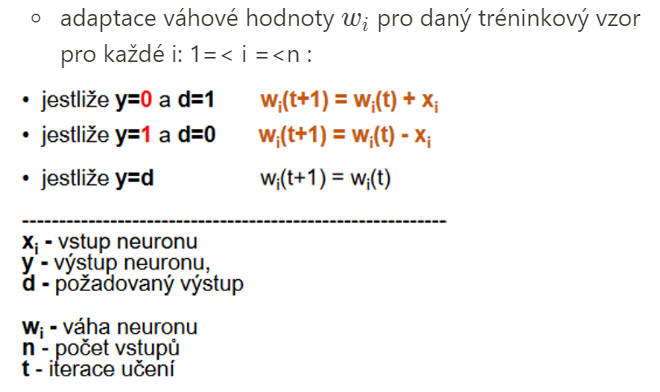
\includegraphics[scale = 0.7]{images/perceptron_vahy1.png}
\end{figure}
B):
\begin{figure}[H]
    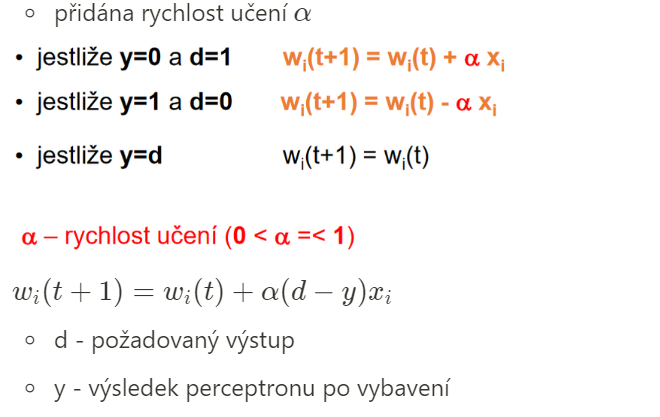
\includegraphics[scale = 0.7]{images/perceptron_vahy2.png}
\end{figure}
C):
\begin{figure}[H]
    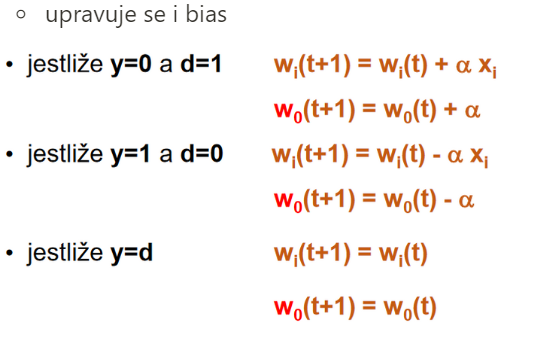
\includegraphics[scale = 0.7]{images/perceptron_vahy3.png}
\end{figure}

\subsubsection{vybavování}
Výstup:
\begin{itemize}
    \item 0/1
    \item -1/1
    \item -1/0/1
\end{itemize}
\subsubsection*{Kritika perceptronu}
schopný řešit jen problémy, které jsou linárně separabilní\\
nelze realizovatfunkci XOR

\subsection{Algoritmus Backpropagation}
Charakteristika
\begin{itemize}
    \item neuron - spojitá přenosová funkce
    \item topologie - vícevrstvá, přímovazební
    \item učení - s učitelem, iterační gradientní proces nastavení vah, algoritmus se zpětným šířením chyby
    \item vybavování - jednorázový proces
    \item aplikace - modelování nelineárních funkcí, klasifikace
\end{itemize}

\subsubsection{Neuron}
ve vstupní vrstvě distribuce signálu, přenosová funkce lineární(nemusí mít strmost 1) \(f(z) = \sigma \cdot z\) \\
ostatní vrstvy přenosová funkce:
\begin{itemize}
    \item sigmoida (výstup 0/1) \(f(z) = \frac{1}{1+e^{-\sigma \cdot z}}\)
    \item tangenta hyperbolická (-1/1) \(f(z) = \frac{1-e^{-\sigma \cdot z}}{1+e^{-\sigma \cdot z}}\)
\end{itemize}

\subsubsection{Topologie}
minimálně 3 vrsty neuronů\\
vstupní vrstva - distribuce signálu\\
prostřední vrstvy(skryté) - úplné propojení neuronů, každý neuron z nižší vrstvy je připojen ke každému neuronu z nižší vrstvy.\\
\begin{figure}[h!]
    \centering
    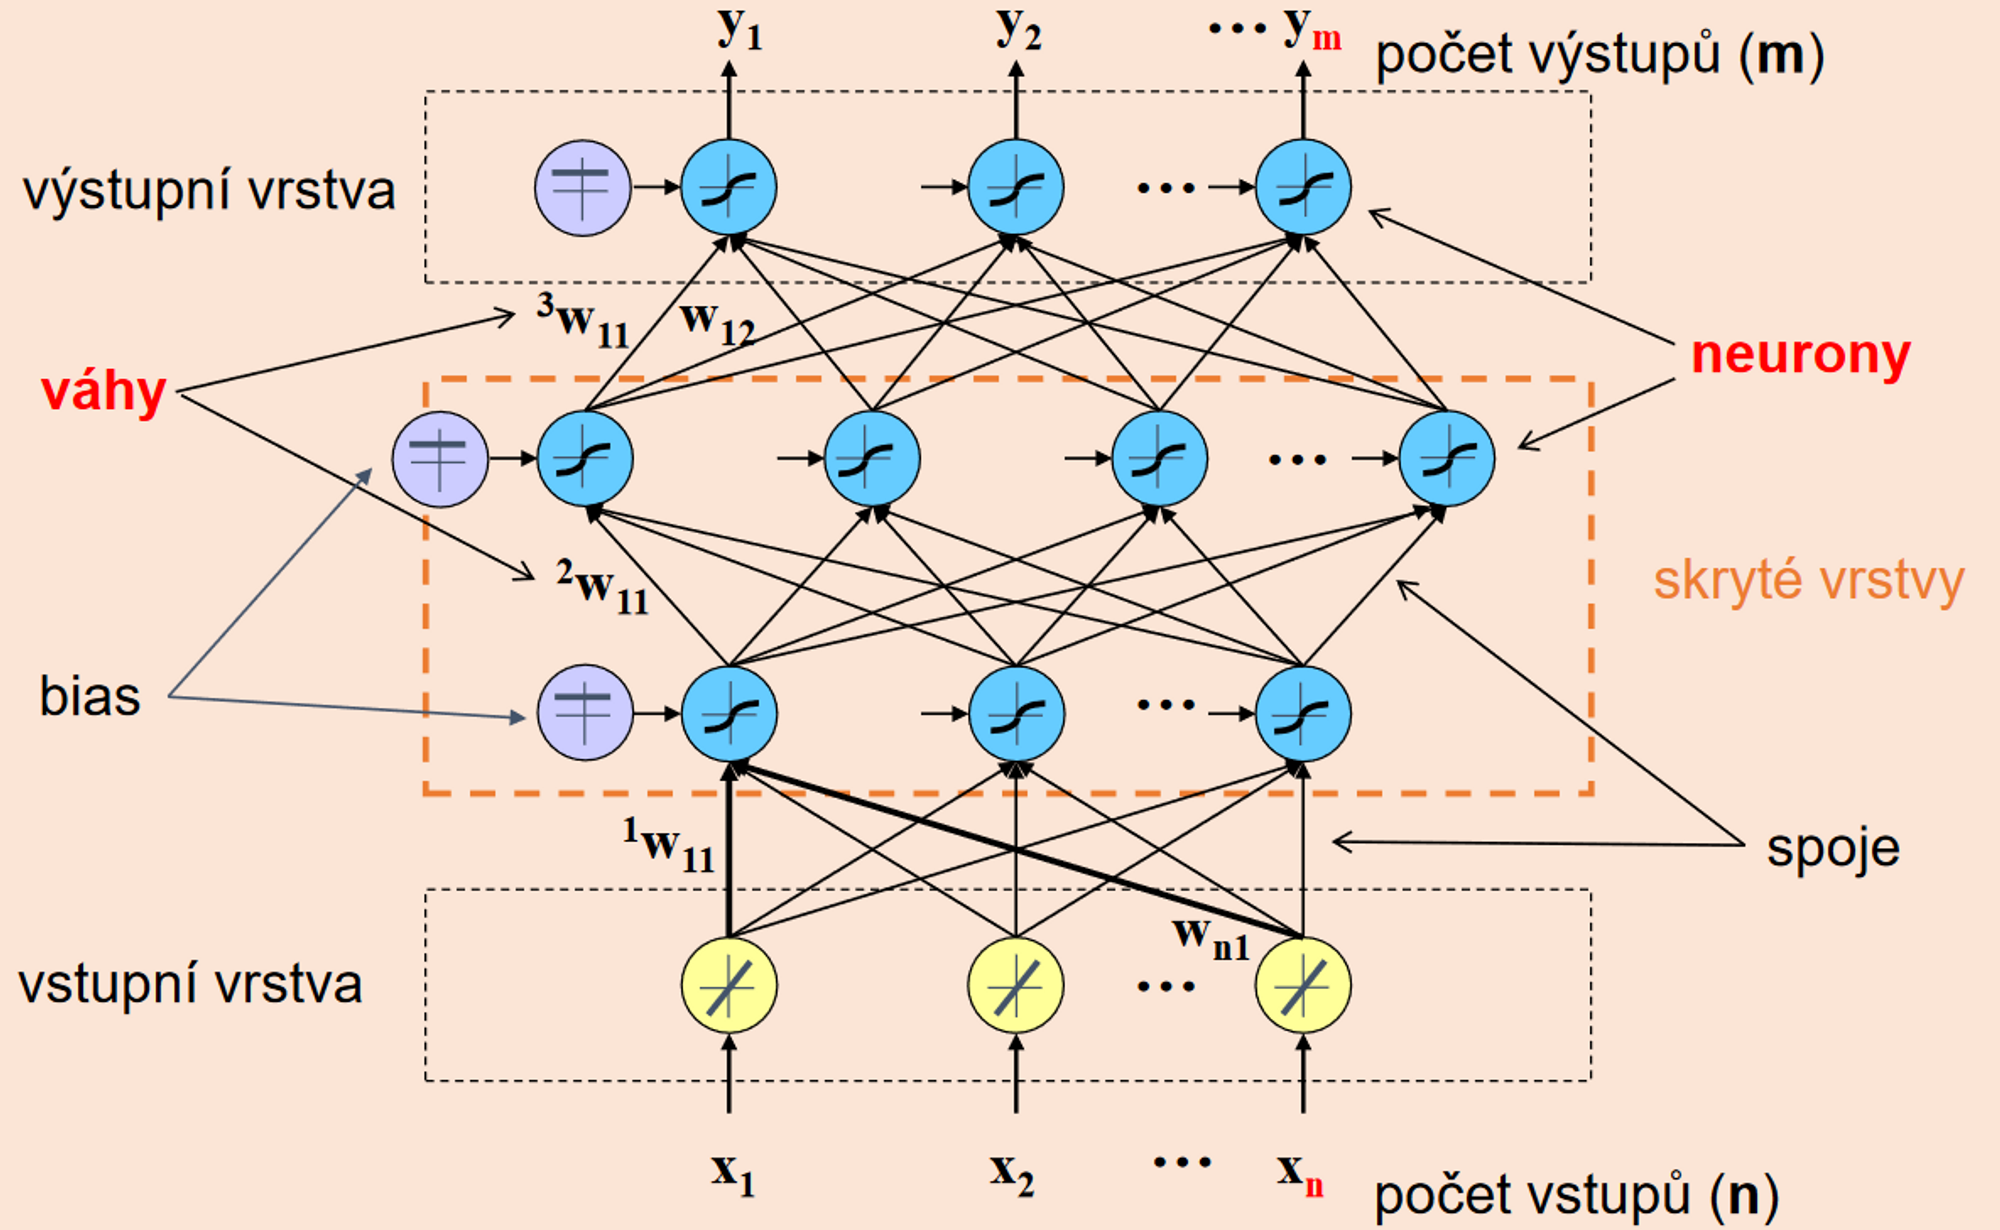
\includegraphics[scale = 0.2]{images/backPropag_topologie.png}
\end{figure}

\subsubsection{Učení}
Učení s učitelem\\
Iterativní gradientní algoritmus, který minimalizuje kvadráty chybové funkce \textit{E}.\\
Chyba sítě \textit{E} představuje rozdíl mezi skutečnými hodnotami \textit{y} a požadovanými hodnotami \textit{d} výstupu neuronové sítě pro danou množinu \textit{T}.\\
\begin{center}
    Chyba vzhledem k s-tému trénikovému vzoru: \(^{s}E = \frac{1}{2}\sum_{j = 1}^{m}(^{s}y_j - ^{s}d_j)^2\)\\
    Celková chyba sítě, součet chyb vzhledem ke tréninkovým vzorům \textit{p}: \(E_c = \sum_{s = 1}^{p} = \frac{1}{2}\sum_{s = 1}^{p}\sum_{j = 1}^{m}(^{s}y_j - ^{s}d_j)^2\)
\end{center}
Adaptace vah - přepočet vah pro minimalizaci celkové chyby:
\begin{center}
    Výpočet nové váhy: \(w_{ij}(t+1) = w_{ij}(t) + \Delta w_{ij}\)\\
    Adaptace váhy na základě chyby: \(\Delta w_{ij} = -\alpha \cdot \frac{\partial E_c}{\partial w_{ij}} = -\alpha \cdot \sum_{s = 1}^{p} \frac{\partial ^{s}E}{\partial w_{ij}}\)
\end{center}
Kroky učení:
\begin{figure}[H]
    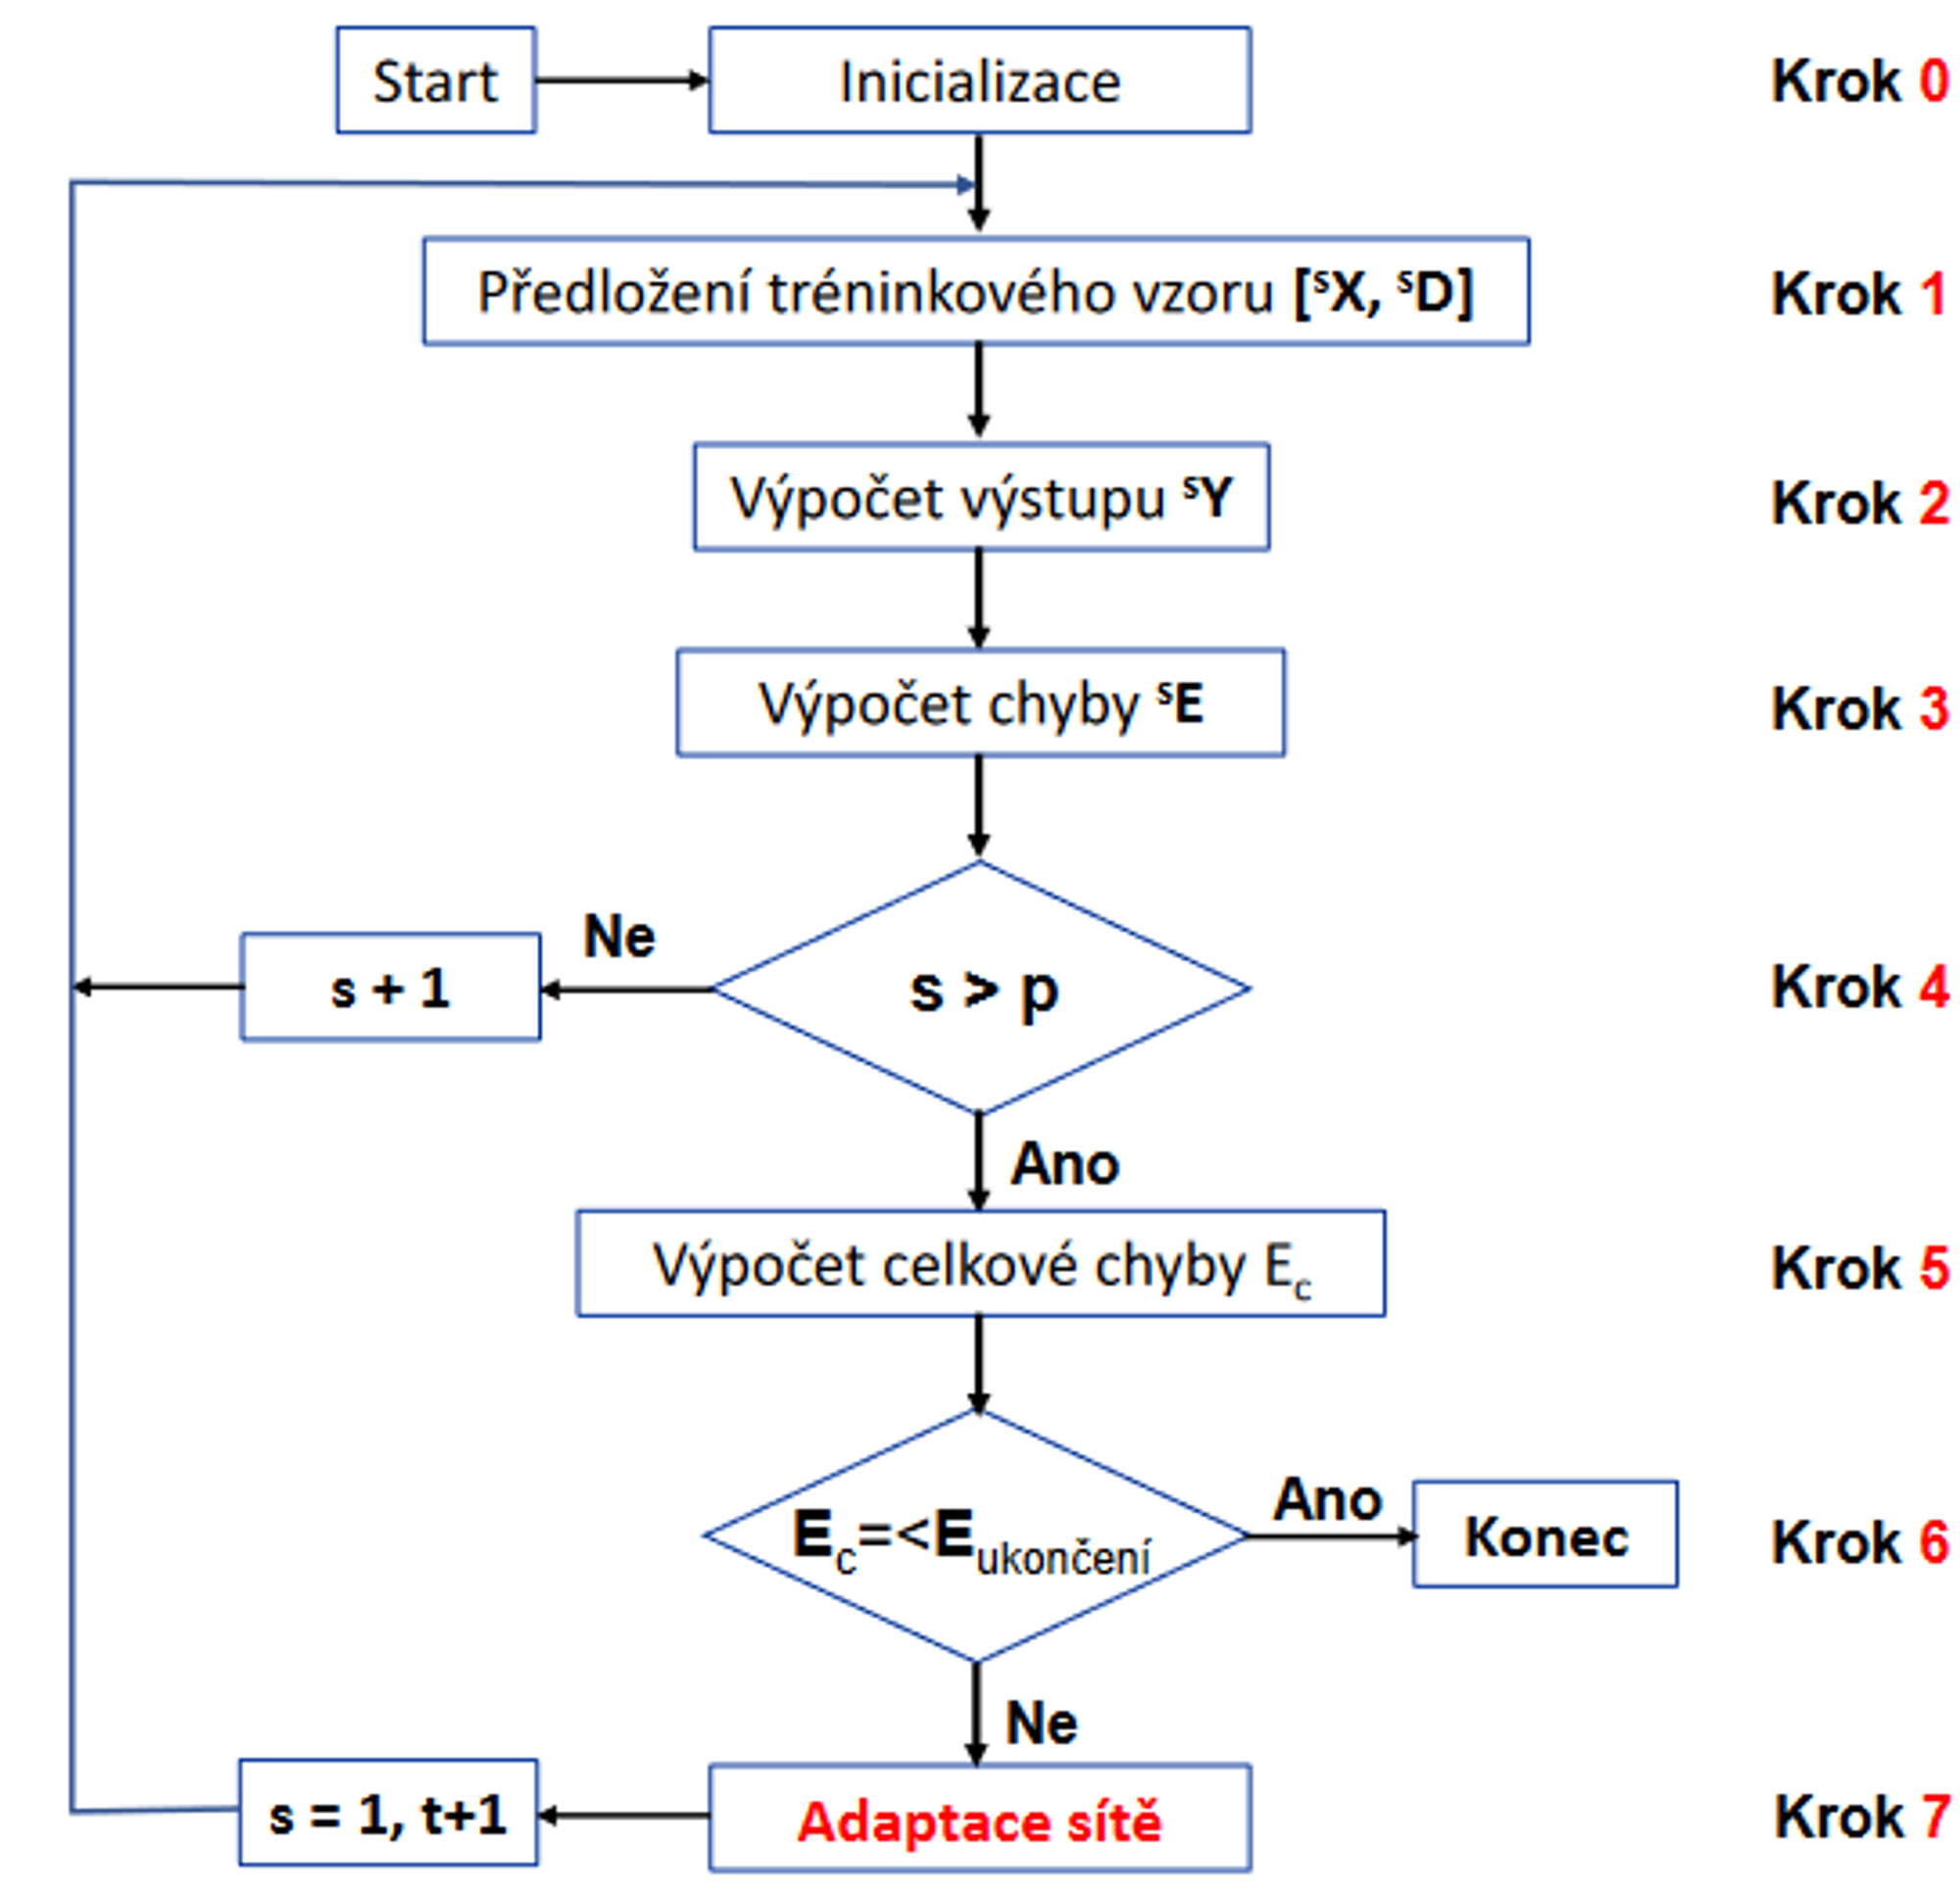
\includegraphics[scale = 0.3]{images/backPropag_uceni.png}
\end{figure}
s \dots počet tréninkových vzorů\\
p \dots celkový počet tréninkových vzorů\\
Akumulované učení - adaptace vah po předložení všech t. vzorů, nezáleží na pořadí vzorů\\
Adaptace po každém tréninkovém vzoru - záleží na pořadí vzorů, zpomaluje konvergenci

\subsection{Kohonenova samoorganizační mapa}
soutěžní strategie učení - aktivní je pouze 1 neuron\\
nástroj pro identifikaci neznámých vlastností a parametrů skrytých ve vstupních datech (rozmisťování zboží podle toho, jak lidi nakupují)\\
K adaptaci vah se využívá statistické vlastnosti tréninkové množiny.\\
Samoorganizační sturktura je taková struktura, která se sama mění podle svých vnitřních pravidel, bez vnějších vlivů.\\
Charakteristika:
\begin{itemize}
    \item neuron - lineární, měření vzdálenosti
    \item topologie - dvouvrstvá s definovaným okolím ve 2.vrstvě
    \item učení - iterační proces, bez učitele
    \item vybavování - jednorázový proces
    \item aplikace - hodně naměřených dat
\end{itemize}
\subsubsection{Neuron}
ve vstupní vrstvě lineární přenosová funkce \(f(z) = z\)\\
ve výstupní není přenosová funkce, zde se provádí výpočet vzdálenosti d předloženého vzoru od vzoru zakódovaného ve vahách neuronu.
\begin{equation}
    d_j = \sum^n_{i=1} \left(x_i - w_{ij}(t)\right)^2
\end{equation}
\subsubsection{Topologie}
Dvouvrstvá síť s úplným propojení neuronů\\
Vstupní vrstva pouze přeposílá informace do výstupní vrstvy.\\
Výstupní vrstva je kompetiční\\
\begin{figure}[H]
    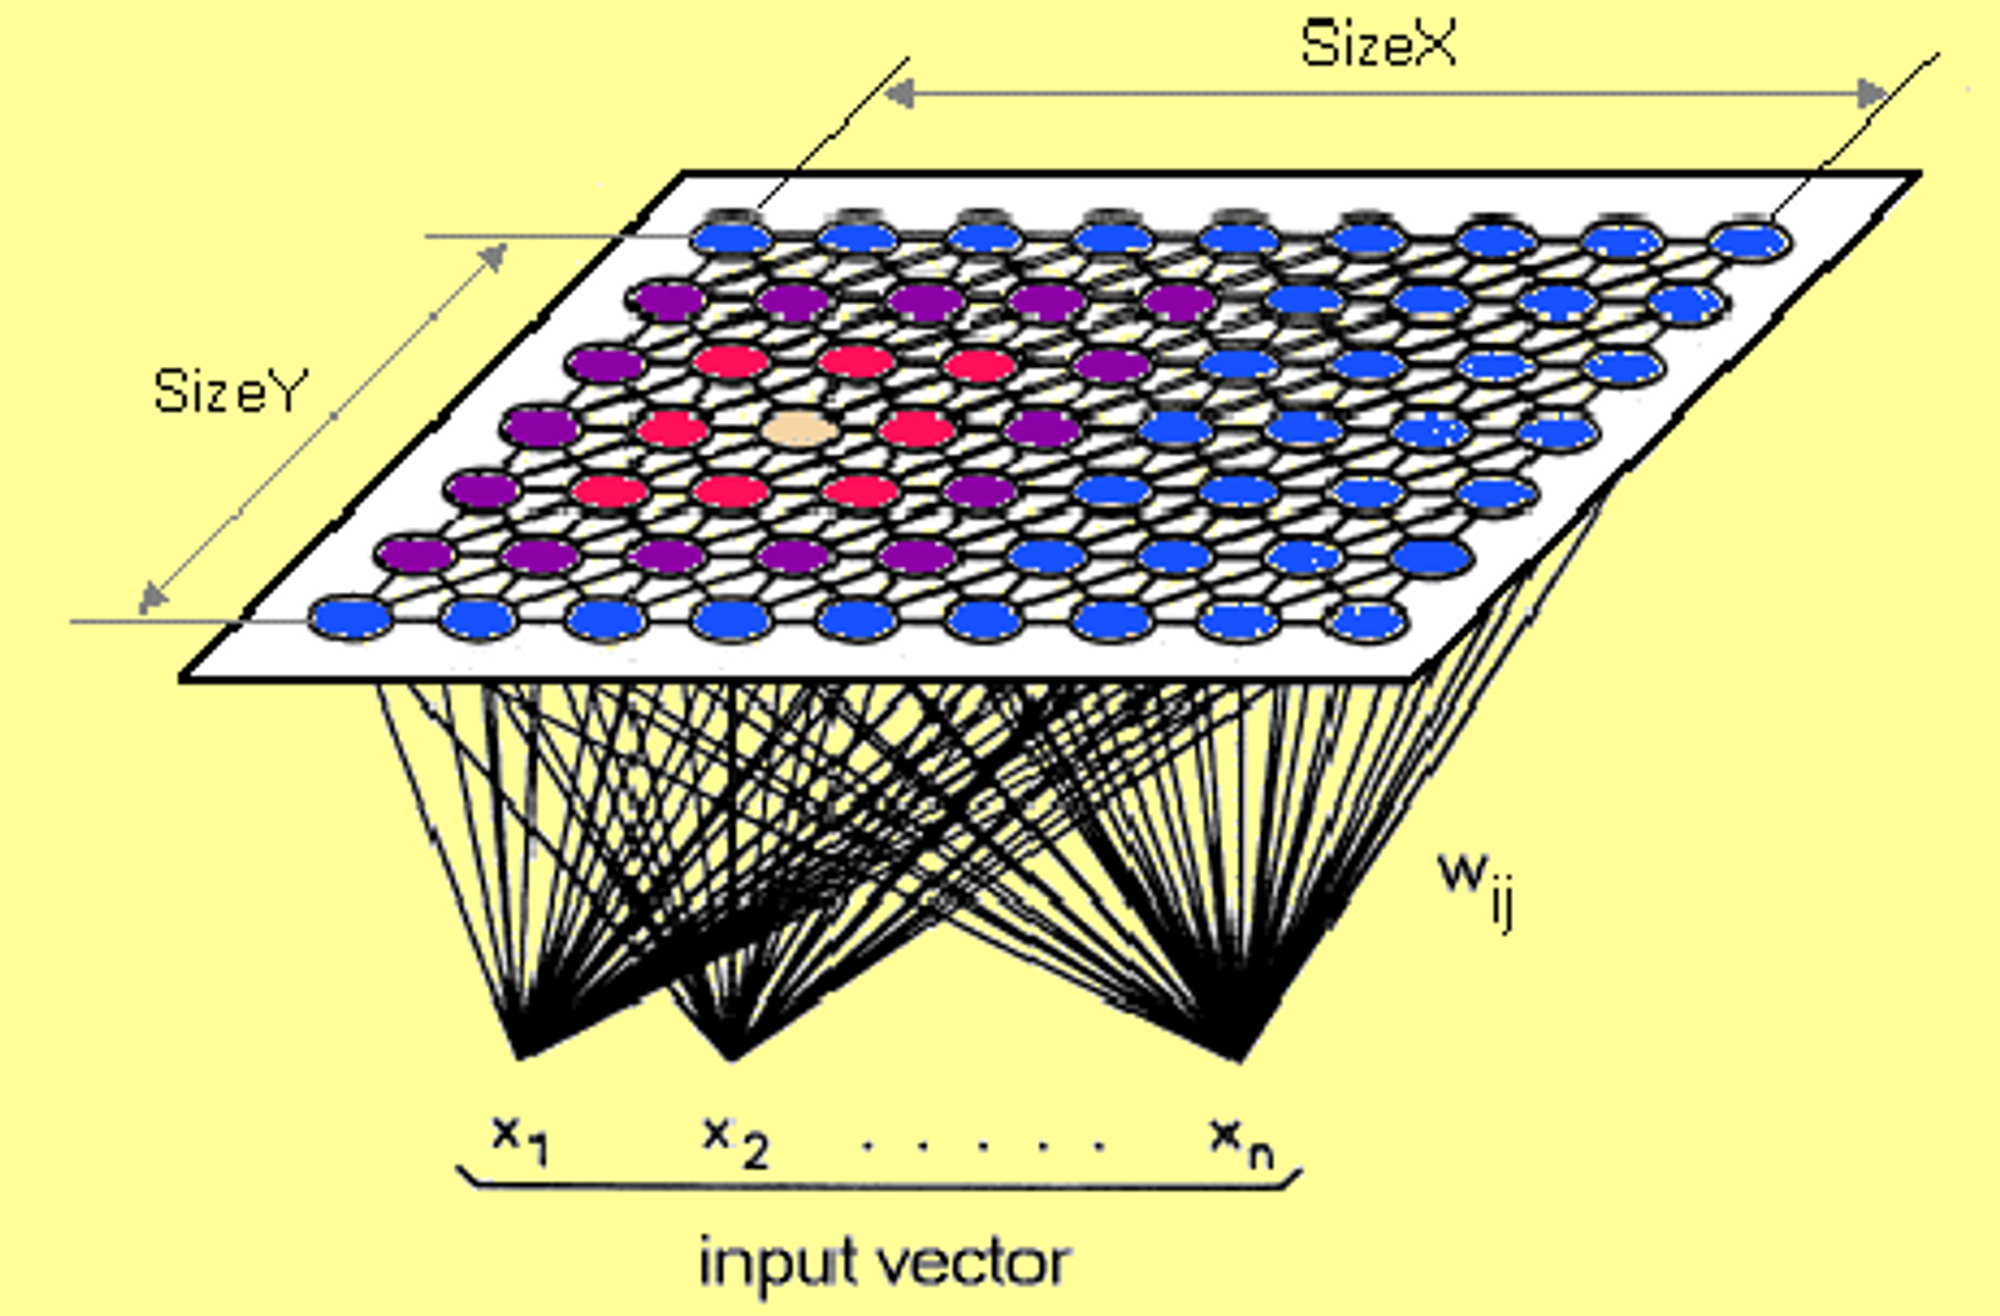
\includegraphics[scale = 0.3]{images/kohonen_topologie.png}
\end{figure}
struktura určuje, které neurony spolu sousedí:
\begin{figure}[H]
    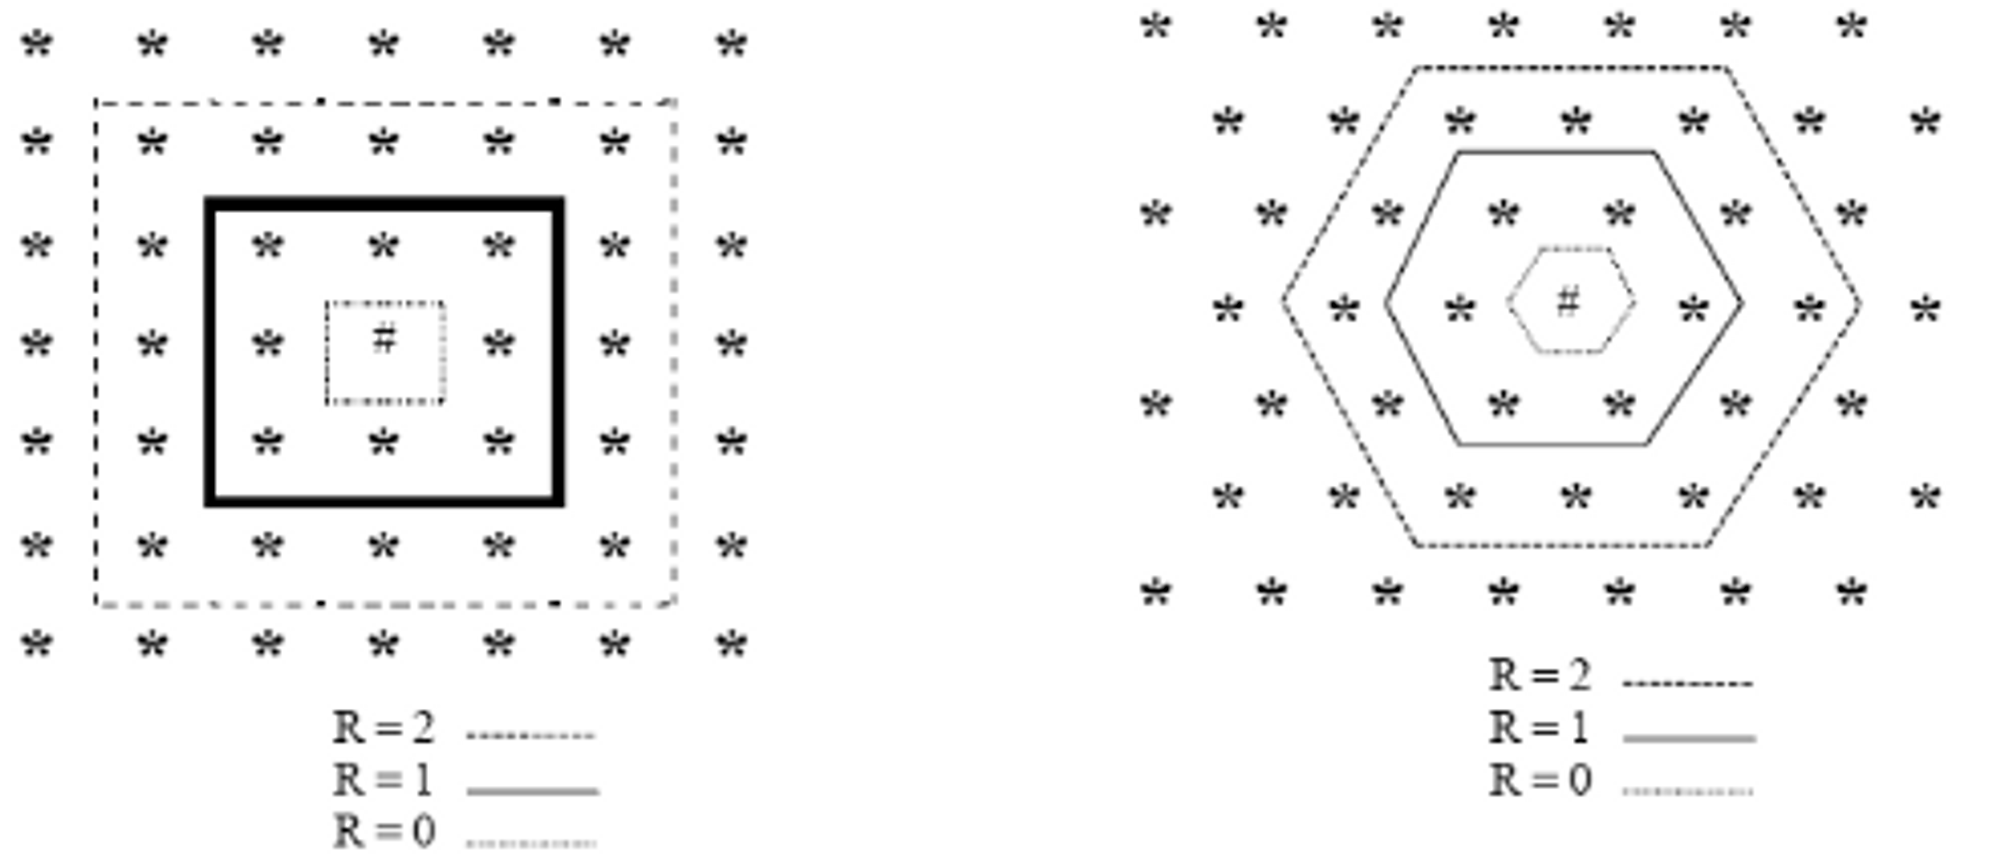
\includegraphics[scale = 0.3]{images/kohonen_struktura.png}
\end{figure}

\subsubsection{Učení}
Iterační bez učitele.\\
Kompetice je proces kdy mezi sebou několik neuronů soutěží a ve fázi učení a u vítězného neuronu se zvýší hodnoty vah a u ostatních se sníží.\\
Vysvětlivky: \(\Phi\) je podmínka ukončení, \(\alpha\) je koeficient učení, \(\rho\) je velikost okolí.\\
\begin{enumerate}
    \item Nastavení topologie: \textit{n} neuronů na vstupu, \textit{m} neuronů na výstupu
    \item incializace: Nastavení vah, koeficientu učení, velikosti okolí, koeficientu ukončení
    \item Předložení tréninkového vzoru z tréninkové množiny
    \item Výpočet vzdálenosti \(d_j\)
    \item Určení vítězného neuronu na základě nejmenší vzdálenosti od tréninkového vzoru: \(d_j = \min(d_j)\), kde \(1 \leq j \leq m \)
    \item Adaptace váhy vítězného neuronu a jeho okolí \(\rho_j(k)\)
    \item Test zda byla projita celá tréninková množina
    \item Aktualizace paramterů: iterace k+1, \(\alpha(k+1) = \alpha(k) - \epsilon\), \(\rho(k+1) = \rho(k) -1 \)
    \item Test ukončení: pokud \(\alpha(k+1) > \Phi\) zpět na krok 2, pokud \(\alpha(k+1) \leq \Phi\) konec učení
\end{enumerate}

\subsubsection{Vybavování}
\begin{enumerate}
    \item předložení vzoru
    \item výpočet vzdáleností
    \item nalezení vítězného neuronu
\end{enumerate}

\subsubsection{aplikace}
\begin{itemize}
    \item zpracování řeči, obrazu
    \item hledání a detekce osob podle fotografií
    \item přepis ručně psaného textu na tištěný
    \item automatické třídění
\end{itemize}
\newpage

\subsection{Konvoluční neuronová síť}
Typické využití u zpracování obrazu.\\
Místo klasického násobení matic, jako je tomu u ANN, využívá CNN konvoluci.\\
Konvoluce je matematická operace, která 2 vstupní funce spojí do jedné výstupní funkce.\\
Má konvoluční jádro, kterým prochází každý prvek obrazu/pole. Velikosti konvolučních jader bývají 3x3 až 11x11\\
Topologie vícevrstvá neuronová síť.\\
Vstupní obraz se musí většinou zkomprimovat pomocí konvoluce a poolingu.\\
Velikost obrazu po projití konvolucí s kernelem:
\begin{center}
    \((N-F)/stride +1\), kde N je délka hrany buněk ve vstupu, N je velikost kernelu a stride je velikost kroku kernelu.\\
    Příklad: Máme obraz o velikosti 7x7, kernel velikosti 3x3 a stride 1:\\
    \((7-3)/1+1 = 5\) Výsledkem bude obraz velikosti 5x5
\end{center}
Další částí v CNN jsou takzvané max pooling vrstvy, ty slouží k redukci dimenzí vstupního signálu bez ztráty jeho informační hodnoty. Funguje tak, že se vezme oblast ve vstupním signálu, z této oblasti se vezme maximální hodnota ta se využije jako informace pro novou redukovanou strukturu. Nejčastěji bývají velikosti 2x2.\\
\begin{figure}[h!]
    \centering
    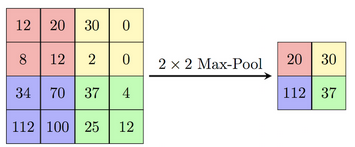
\includegraphics[scale = 0.5]{images/MaxPooling.png}
\end{figure}

Princip: Je založené na feature extraction ze vstupu pomocí velkého množství malých kernelů. Nižší vrstvy extrahují geometrické tvary(edge detectors), vyšší vrstvy detekují komplexnější struktury. Výsledek je na konci zpracovaný pomocí Fully-Connected Neural Network.\\
Aktivační funkce:
\begin{itemize}
    \item sigmoid
    \item tanh \(f(x) = \frac{e^{2x}-1}{e^{2x}+1}\)
    \item ReLU - Rectified Linear Unit - prakticky jenom říká, že pokud je hodnota funkce f(x) menší jak 0, pak ji nastaví na 0, pokud je větší tak se ponechá hodnota funkce.
    \item Leaky ReLU - založná na ReLU, ale místo nastavení záporných hodnot do 0, je ponechá záporné, ale pomocí konstanty snižuje jejich sklon
    \item softmax - aktivační funkce pro klasifikaci do tříd. Vrací pravděpodobnosti toho jak je pravděpodobné, že vstupní objekt patří do některé z výstupních tříd. Pokud máme \textit{N} výstupních tříd, pak výsledkem softmax bude vektor délky \textit{N}, kde na každém indexu \textit{i} bude pravděpodobnost  zobrazena číslem v intervalu \(<0;1>\). Softmax se počítá jako \(softmax(z)_i = \frac{e^{z_i}}{\sum_{j = 1}^{N}e^{z_j}}\), kde \textit{e} je eulerovo číslo, \textit{z} je vektor vstupních hodnot, i je index prvku vstupního vektoru \textit{z}. Tedy celková funkce softmax je založena na kalkulaci exponentu pro každý prvek \textit{z}, vydělit jej sumou všech exponentů a následně je umístit do výsledného vektoru pravděpodobností.\\
\end{itemize}
\begin{figure}[h!]
    \centering
    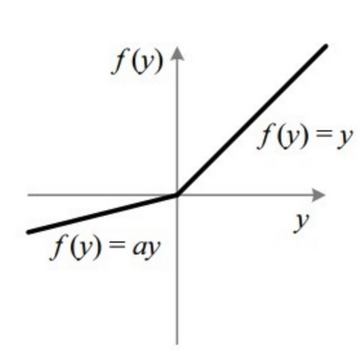
\includegraphics[scale = 0.3]{images/LeakyReLU.png}
    \caption{Leaky ReLU}
\end{figure}

Overfitting je případ kdy se neuronová síť přespříliš adaptuje na vstupní množinu dat a ztrácí generalizaci, tudíž není schopná zařadit nová data, která nebyly v trénovacím datasetu.\\
Batch learning je proces kdy neupravujeme váhy v neuronové síti s každou iterací, ale místo toho akumulujeme všechny změny vah pro tréninkové vzory a poté se nové váhy spočítají průměrem z těchto změn vah, to vede ke snížení overfittingu pro určitá data.\\

\begin{figure}[H]
    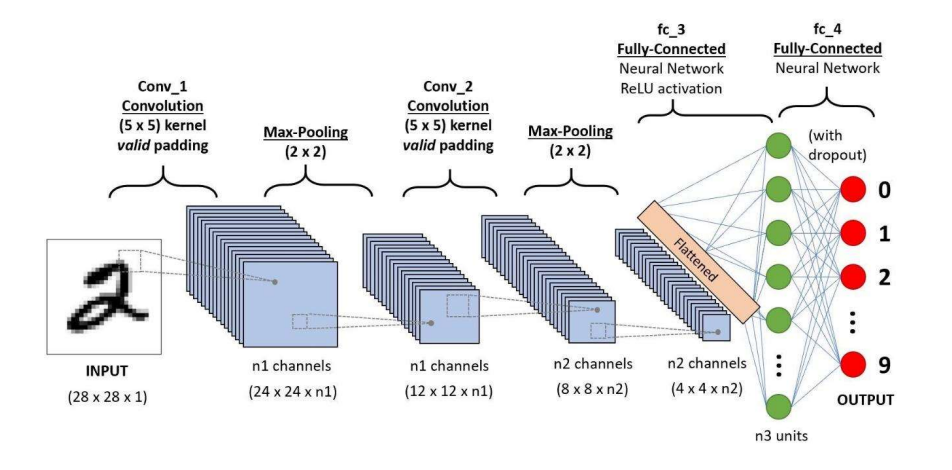
\includegraphics[scale = 1]{images/konvoluce.png}
\end{figure}
\newpage

\section{Expertní systémy(ES) - definice, architektura, teoretické zdroje pro realizaci ES, tvorba a ladění báze znalostí, průběh konzultace}
Počítačové programy, které simulují rozhodovací činnost experta při řešení velmi složitých úloh a využívají vhodně zakódovaných speciálních znalostí převzatých od experta\\
ES jsou využívány tam, kde neexistuje dostatečné algoritmické řešení a jediným možným řešením je určitá forma usuzování.\\
Charakteristické rysy:
\begin{itemize}
    \item neurčitost v bázi znalostí
    \item neurčitost v odpovědích uživatele
    \item dialogový režim
    \item vysvětlovací činnost
    \item modularita a transparentnost báze znalostí
\end{itemize}
Modularita umožňuje lehce aktualizovat bázi znalostí. Transparentnost zajišťuje lehkou čitelnost, srozumitelnost a ovládání.\\
\subsection{Role ES}
asistent - pomůcka experta na potvrzení či zpochybnění svých profesionálních názorů\\
kolega - expertní systém navrhuje řešení, konečné rozhodnutí dělá uživatel\\
expert - pracuje úplně autonomně na úkolech, které uživatel není schopen vyřešit\\

\subsection{Architektura}
Zjednodušenná verze:
\begin{figure}[H]
    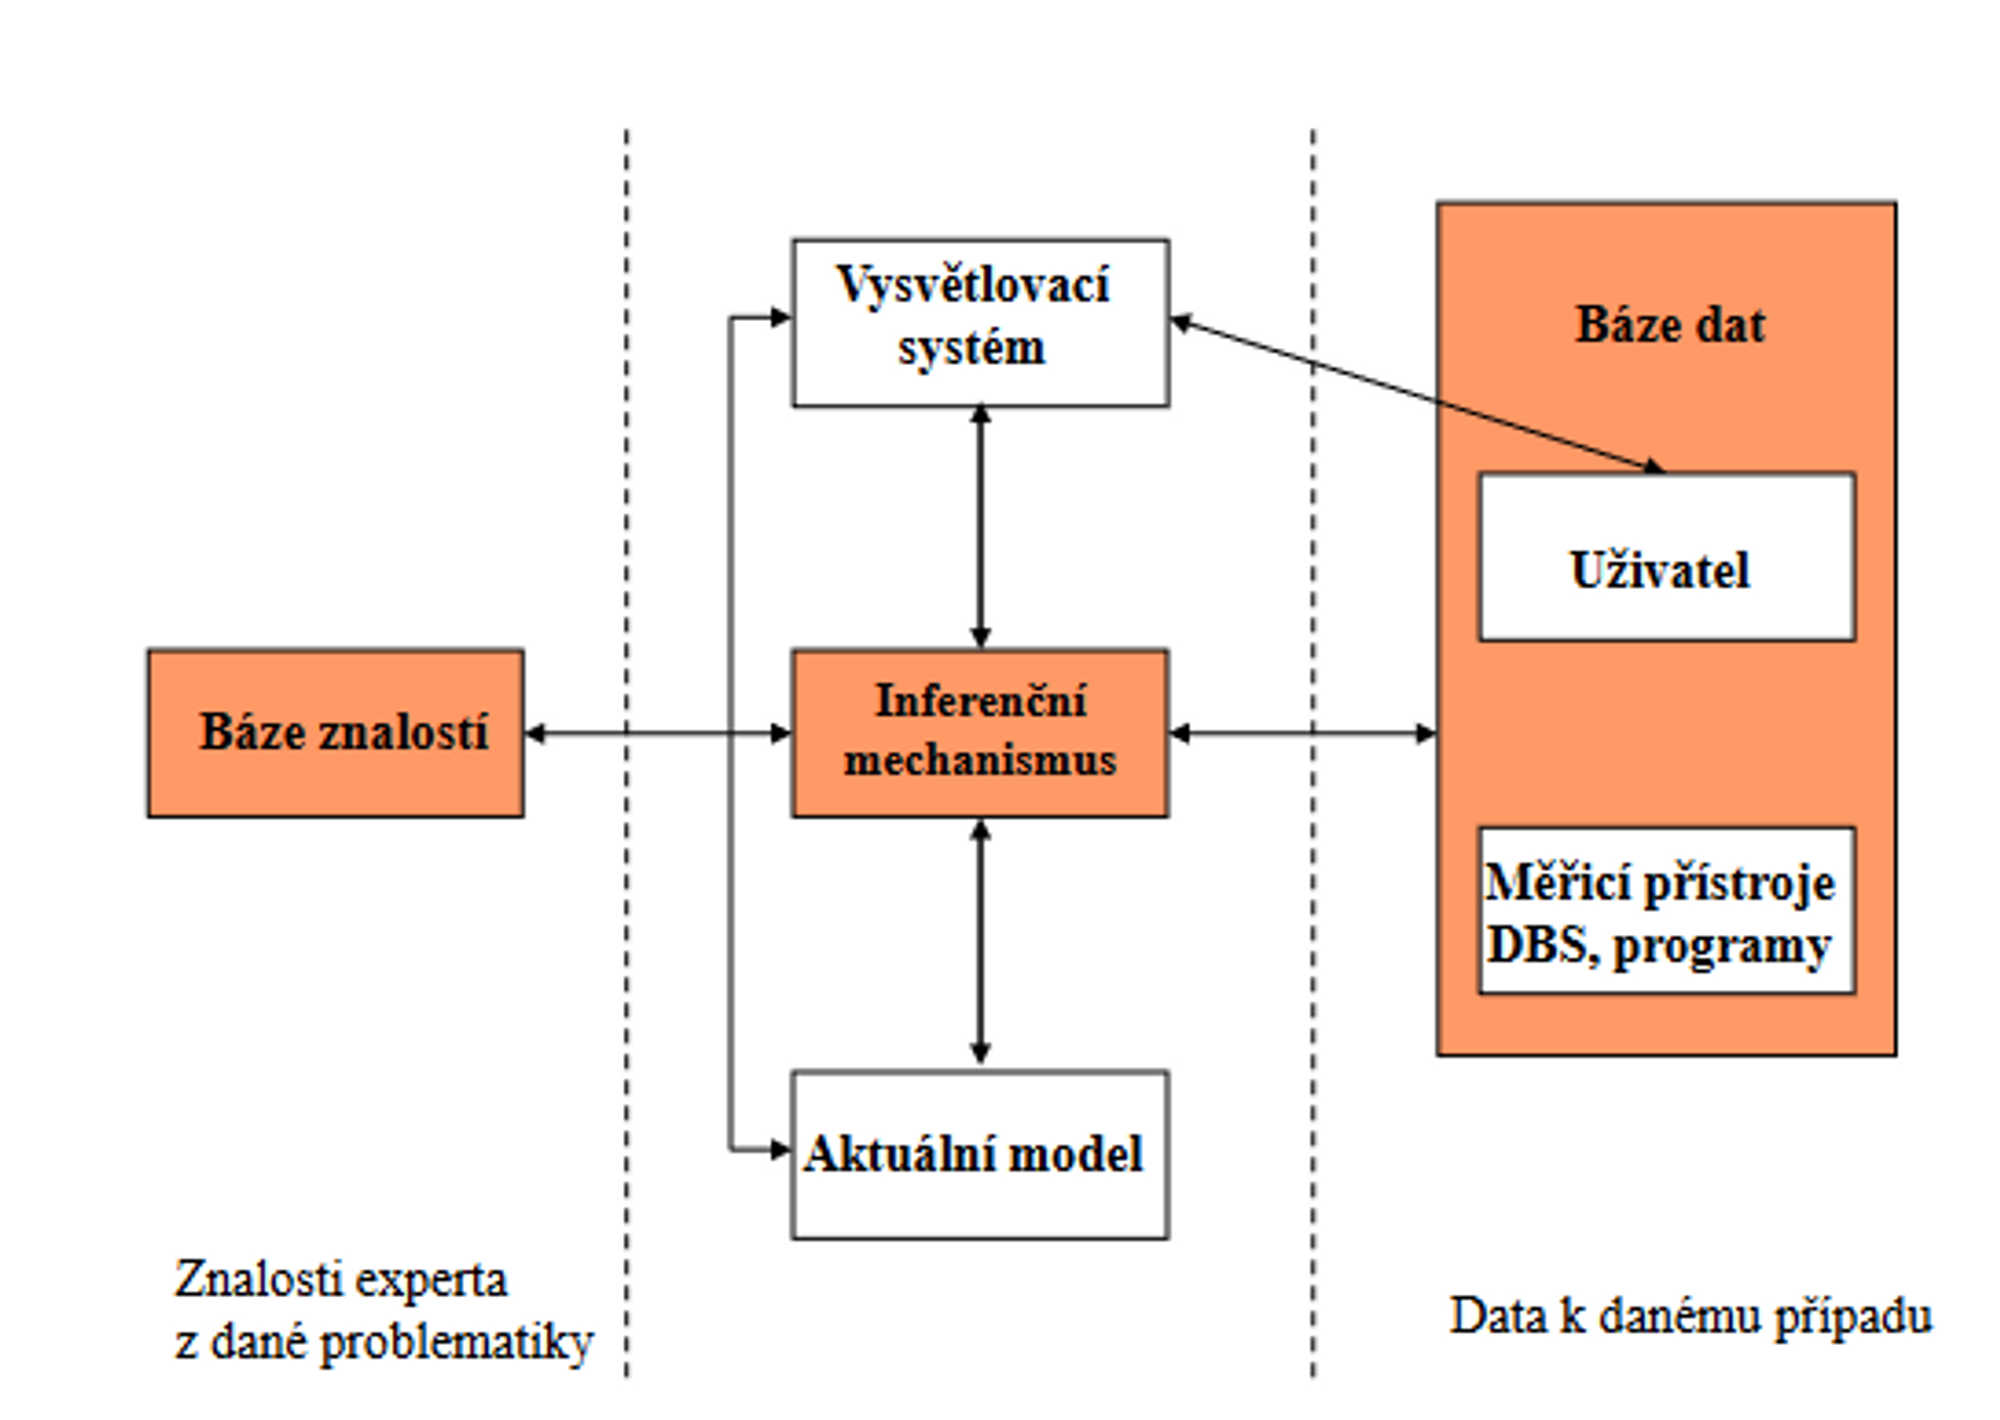
\includegraphics[scale = 0.3]{images/ES_ez.png}
\end{figure}
Inferenční mechanismus
\begin{itemize}
    \item Zajišťuje komunikaci s uživatelem prostřednictvím uživatelského rozhraní - dialogový režim
    \item obsahuje obecné algoritmy schopné řešit problémy na základě manipulace se znalosti z báze znalostí
    \item určuje jak a v jakém pořadí aplikovat pravidla na bázi dat
    \item založen na inferenčním pravidle odvozování nových poznatků nebo na prohledávání báze znalostí
\end{itemize}
Báze znalostí - vytváří se v průběhu řešení konkrétního problému a obsahuje data k řešenému problému\\
Aktuální model - reprezentace současného stavu řešení - v průběhu konzultace vyjádřen pravděpodobností\\
vysvětlovací modul - vysvětlení položené otázky,zdůvodňuje postup při řešení problému, odlišuje ho od znalostního systému

\subsection{Typy ES}
Obecné rozdělení:
\begin{itemize}
    \item 90\% - diagnostický
    \item 9\% - generativní/plánovací
    \item 3\% - dedikovaný/smíšený
\end{itemize}
Podle obsahu báze znalostí:
\begin{itemize}
    \item prázdný
    \item naplněná
\end{itemize}

Diagnostický:
\begin{itemize}
    \item úkolem určit, která hypotéza nejlépe koresponduje s daty týkající se daného případu
    \item pracují s pevným počtem cílů, z nichž vybírají svá doporučení
\end{itemize}
Plánovací
\begin{itemize}
    \item je znám počáteční stav a cíl řešení
    \item cíl nalézt posloupnost kroků, který k cíli dovede
    \item znalost experta + data: omezené množství řešení
\end{itemize}

Smíšený - funguje na základě střdání jednotlivých přístupů podlde potřeby\\

\subsection{Teoretické zdroje}
Reprezentace znalostí
\begin{itemize}
    \item Deklarativní - jednotlivá fakta
    \item proceduální - znalosti ve formě procesů
    \item pravidla, rozhodovací stromy
\end{itemize}
Řešení úloh a prohledávání stavového prostoru(inferenční mechanismus)
\begin{itemize}
    \item prohledávání stavového prostoru
    \item rozklad na podproblémy
    \item dedukce - odvození závěru z předpokladu
    \item abdukce - usuzování ze závěru k předpokladu
    \item indukce - postup od specifického případu k obecnému
\end{itemize}
Zpracování neurčité informace
\begin{itemize}
    \item neurčitost - nejisté znalosti, vágní pojmy, nekonzistence dat
    \item fuzzy logika
\end{itemize}

\subsection{Tvorba a ladění báze}
\subsubsection{Identifikace problému}
musí se jednat o problém složitý rozsahem nebo neurčitostí vztahů, pro nějž exaktní metoda řešení není\\
provede se analýza požadavků, nalezení klíčových slov a specifikace vztahů mezi nimi

\subsubsection{Návrh koncepce}
stanovení cíle a funkce systému\\
identifikace možných zdrojů znalostí\\
ucelená představa rozkladu na dílčí úlohy\\

\subsubsection{Volba reprezentace znalostí}
rozhodování o typu formální prezentace znalostí na základě identifikace problému\\
viz reprezentace znalostí\\

\subsubsection{Získávání znalostí}
interview experta nebo automatizované získávání znalostí(strojové učení)\\
mohou nastat problémy - expert nepsolupracuje, výrazy srozumitelné jen lidem v oboru\\

\subsubsection{Implementace}
proces naplňování báze znalostí\\

\subsubsection{Ladění báze}
změna struktury grafu\\
nastavení pravděpodobnostních uzlů na základě testovacích konzultací\\

\subsection{Průběh konzultace}
Má 4 fáze:
\begin{enumerate}
    \item Výběr dotazu - signifikantnější dotazy na začátek
    \item Výběr odpovědi - odpovědi v několika stupních, ovlivňují hypotézy
    \item přepočet báze znalostí - přepočet pravděpodobností
    \item ukončení - na přáni uživatele, nebo byly tázány všechny dotazy
\end{enumerate}

\section{Počítačové vidění - předzpracování obrazu, segmentace obrazu, popis a klasifikace obrazu}
\begin{figure}[H]
    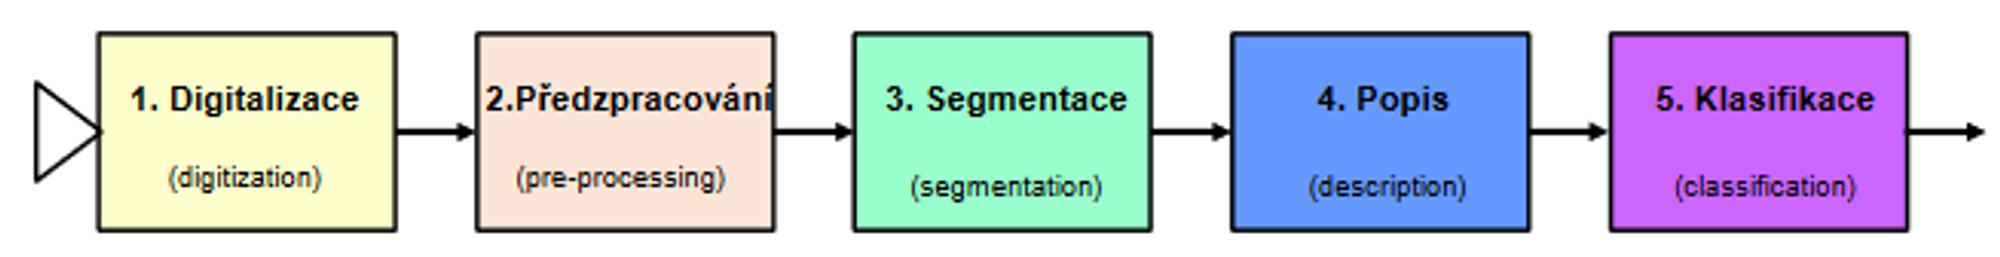
\includegraphics[scale = 0.4]{images/pc_videni.png}
\end{figure}
\subsection{Digitalizace}
Matematická funkce, dvou nebo více argumentů. Obrazová fce: \(f(x,y)\), spojitá v čase: \(f(x,y,t)\).\\
Hodnoty obrazové funkce: jas(BW obraz), RBG(barevný obraz), teplota(termovize), schopnost pohltit záření(rentgenový tomograf).\\
Diskrétní obrazová funkce \(f(x,y)\) je matice pixelů, hodnota pro BW obraz 0 je černá barva, 255 bílá.\\
Pomocí vzorkování v matici MxN bodů, kvantování spoijité jasové úrovně každého vzorku do k intervalů. Vzorkování je rozložení bodů v ploše \(g_s = g(x,y)\cdot s(x,y)\), kde \textit{g} je spojitý obraz a \textit{s} je vzorkovací funkce. Kvantování je převod spojité hodnoty jasové funkce v daném vzorku do příslušného číselného údaje z intervalu jasových hodnot.\\
Obrazový šum jsou velké změny hodnoty jasových hodnot sousedních bodů, vzniká během snímání, zpracování nebo přenosu. Typy šumu: aditivní, multiplikativní, pepř a sůl.\\

\subsection{Předzpracování obrazu}
Cíle:
\begin{itemize}
    \item potlačit šum
    \item odstranit zkreslení
    \item potlačit či zvýraznit jiné rysy obrazu
\end{itemize}
Předzpracováním nezískáme žádnou novou informaci.\\
Metody předzpracování:
\begin{itemize}
    \item bodové jasové transformace
    \item geometrické transformace
    \item lokální předzpracování
    \item obnovení obrazu
\end{itemize}

\subsubsection{Bodové jasové transformace}
Závisle na pozici:
\begin{itemize}
    \item zdroj poruch vzniklý při digitalizaci a přenosu obrazu
    \item systematické chyby lze potlačit na základěznalosti odchylky citlivosti každého bodu od ideální převodní charakteristiky:
          $f(i,j) = e(i,j)\cdot g(i,j)$\\
          Násobíme degradačním koeficientem g
\end{itemize}
\newpage
Nezávislé na pozici:
\begin{figure}[H]
    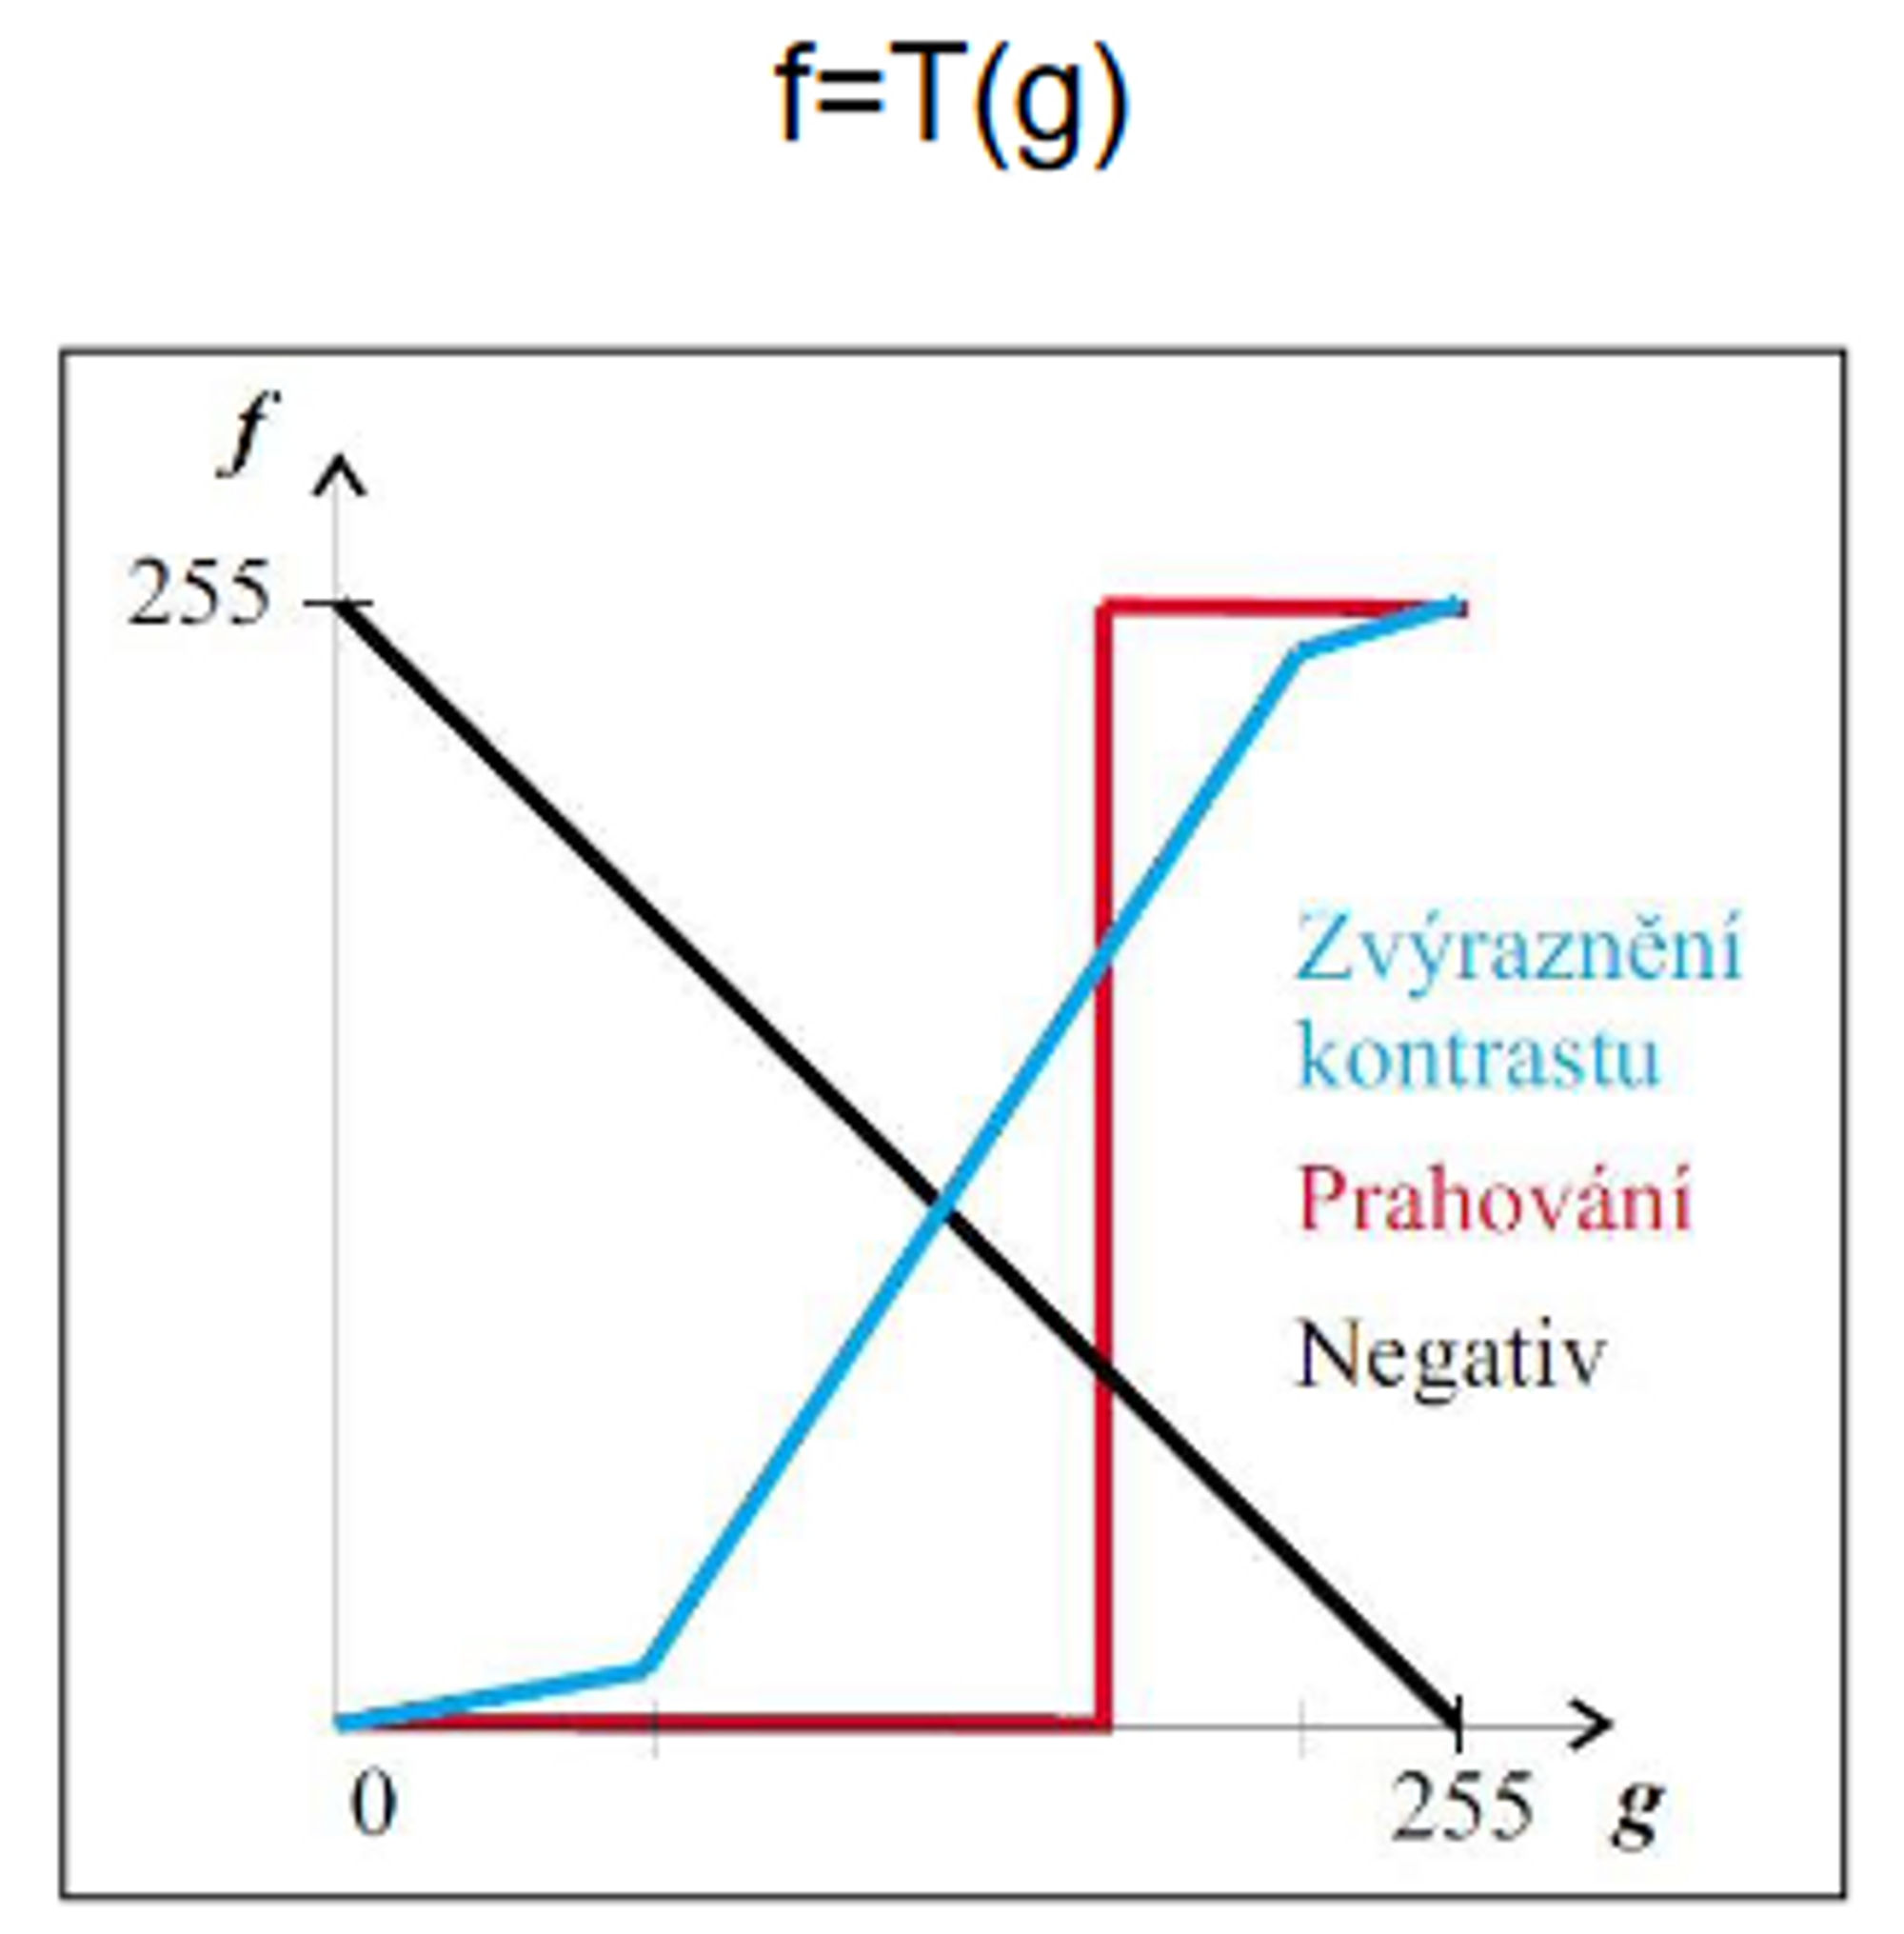
\includegraphics[scale = 0.13]{images/transf_krivka.png}
\end{figure}

\subsubsection{Geometrické transformace}
Používají se k odstranění geometrických zkreslení.\\
Dva kroky:
\begin{itemize}
    \item plošná transformace
    \item jasová transformace
\end{itemize}
Plošná transformace:
\begin{equation}
    x' = \sum_{r =0}^m \sum_{k=0}^{m-r}a_{rk}x^ry^k, \;\;\;\; y' = \sum_{r =0}^m \sum_{k=0}^{m-r}b_{rk}x^ry^k
\end{equation}
dvojce sobě odpovídajících bod x,y a x',y'\\
Jasová transformace:
Přiřazení bodu (x,y) hodnotu jasu nejbližšího bodu v diskrétní mřížce\\
Druhá možnost je určení hodnoty poměrem vzdáleností nejbližších bodů.\\
\newpage
\subsubsection{Lokální předzpracování}
Za účelem filtrace šumu, detekce hran, nebo ostření obrazu.\\
Filtrace:
\begin{itemize}
    \item průměrování
    \item konvoluční maska
    \item metoda mediánem
\end{itemize}
\begin{figure}[H]
    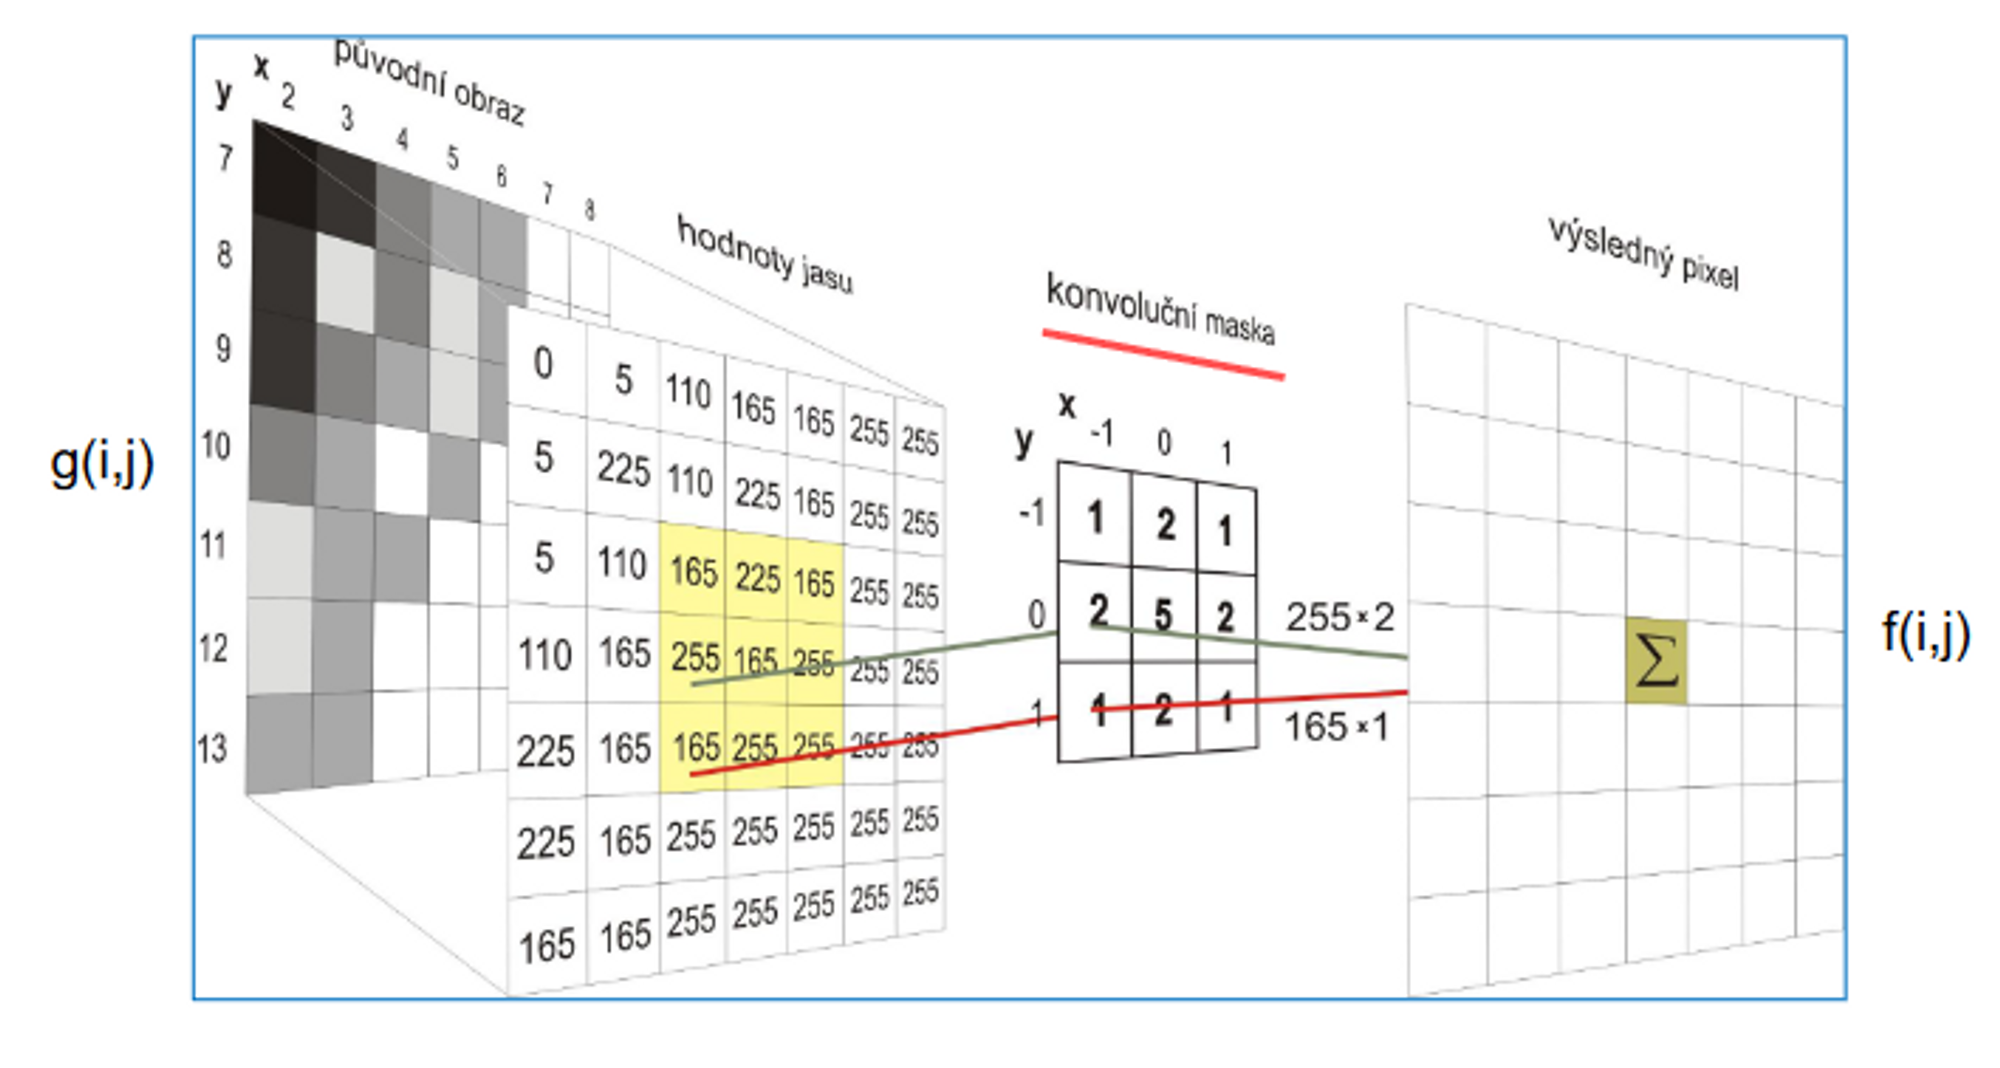
\includegraphics[scale = 0.25]{images/konvoluce_maska.png}
\end{figure}

Detekce hran:
\begin{itemize}
    \item pomocí derivačních filtrů - 1. a 2. derivace
    \item gradientní operátory
    \item laplaceovy operátory
\end{itemize}
\begin{figure}[H]
    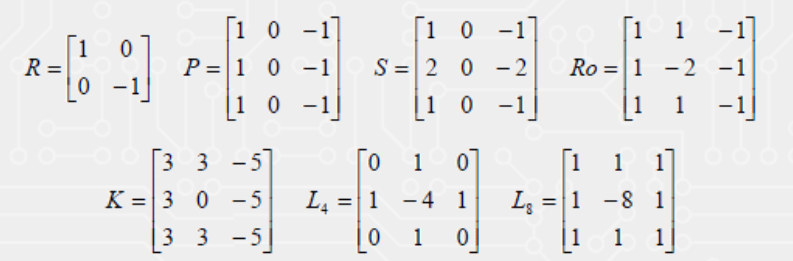
\includegraphics[scale = 0.7]{images/hrany.png}
\end{figure}
Robertsův, Prewittové, Sobelův, Robinsonův\\
Kirschův, Laplaceuv(čtyřokolí, osmiokolí)\\

\subsubsection{Obnovení obrazu}
rozostření objektivu, rozmazání pohybujícícho se objektu\\

\subsection{Segmentace}
Snaha rozčlenit obraz do oblastí, které mají úzkou souvislost s předměty či oblastmi reálného světa zachyceného na obrazu.\\
výsledek je soubor vzájemně nepřekrývajících se oblastí.\\
dělí se na:
\begin{itemize}
    \item kompletní - oblasti jednoznačně korespondují s objekty vstupního brazu
    \item částečná - oblasti nemusí přímo korespondovat s objekty, jsou homogenní vůči nějaké vlastnosti(jas, barva, odrazivost)
\end{itemize}
Cíl připravit data pro popis a redukovat objem dat.\\
Metody:
\begin{itemize}
    \item prahování
    \item detekce hran
    \item segmentace narůstání oblastí
          \begin{itemize}
              \item spojování oblastí
              \item štěpení oblastí
              \item štěpení a spojování oblastí
          \end{itemize}
    \item srovnání se vzorem
\end{itemize}
\begin{figure}[H]
    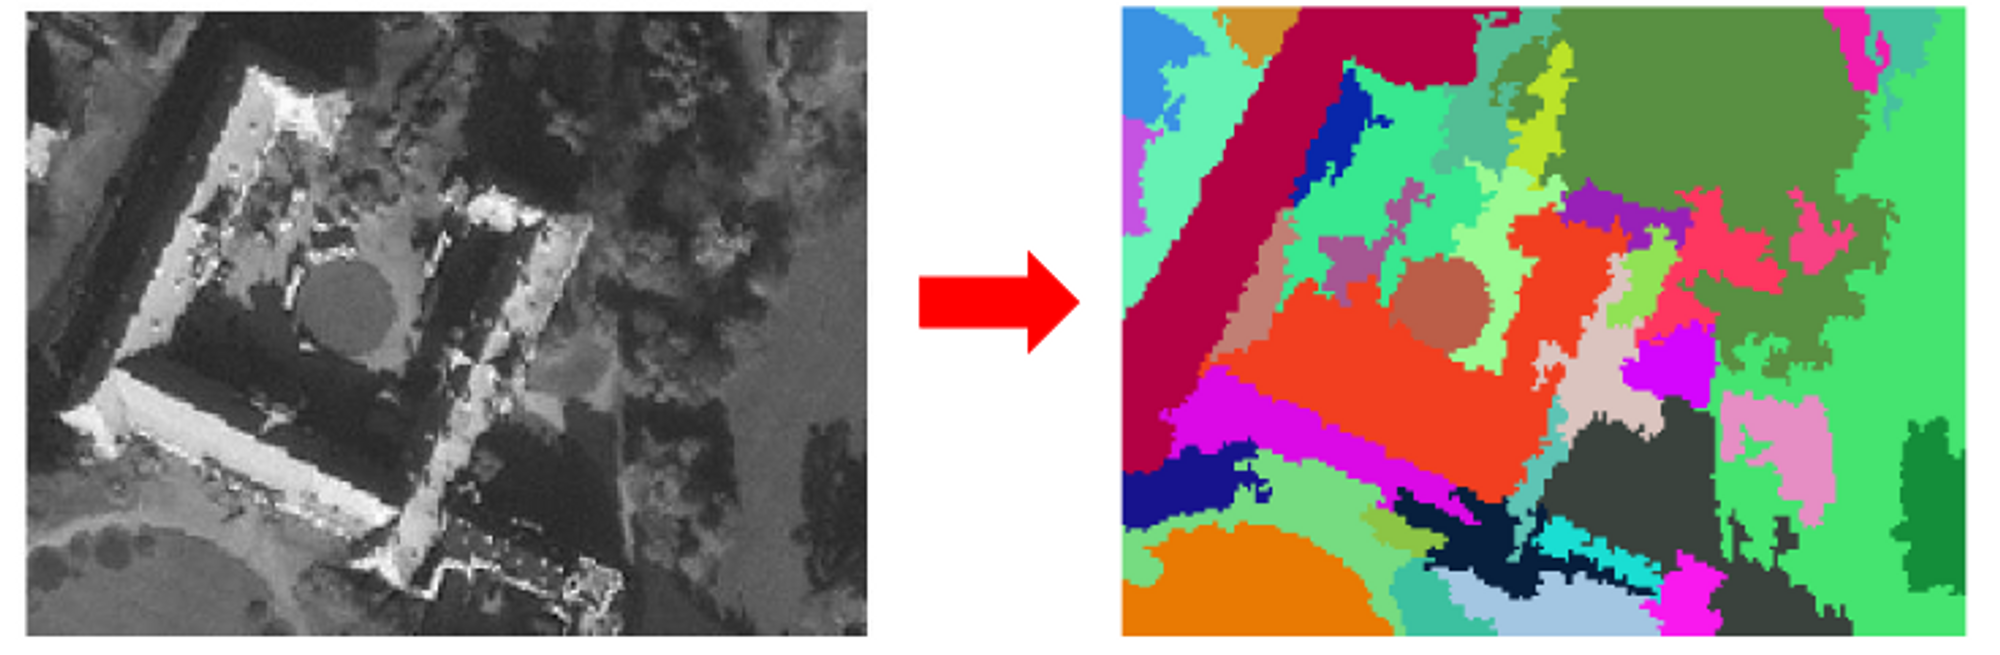
\includegraphics[scale = 0.3]{images/segmentace.png}
\end{figure}

\subsubsection{Prahování}
Vychází z toho, že objekt a pozadí mají rozdílné vlastnosti.\\
Vychází z toho, že mnoho objektů či oblastí obrazu je charakterizováno konstantní odrazivostí či pohltivostí svého povrchu.\\

\subsubsection{Detekce hran}
Hranice objektů se tvoří z hran nalezených pomocí hranových detektorů.\\
Prahování obrazu hran vychází z obrazu velikosti gradientu, který je prahovaný vhodným prahem. Odstrańuje bezvýznamné hrany. Zpracování výsledku pomocí vypuštění všech hran, které nesplňují určitou velikost.\\
Relaxace hran je vytváření souvislých hranic. Při konstrukci se uvažuje s vlastnosti každé hranu, v kontextu hran, které se vyskytují v jejím okolí. Vlastnosti hran se iterčně zpřesňují až dokud není hranový objektu přesný.\\

\subsubsection{Segmentace narůstání oblastí}
Spojování oblastí:
\begin{itemize}
    \item počáteční rozdělení obrazu do velkého množství malých oblastí
    \item defnice kritéria spojování
    \item spojování sousedních oblastí na základě kritéria
\end{itemize}
Štěpení oblastí:
\begin{itemize}
    \item opak spojování
    \item postupné rozkládání obrazu na menší části
\end{itemize}
Štěpení a spojování oblastí:
\begin{itemize}
    \item pyramidální reprezentace obrazu
    \item je-li oblast v dané úrovni pyramidy nehomogenní, je rozštěpena na 4 podoblasti
    \item jsou-li oblasti navzájem homogenní a lze je ve vyšší úrovni spojit do jedné, jsou spojeny
\end{itemize}

\subsection{Popis}
Snaha určit příznaky(vzor, číselný vektor) nebo primitiva(nečíselný syntaktický popis) obrazu.\\
Popis musí být být invariantní proti - posunutí, měřítku, natočení, jasu a šumu.\\
\subsubsection{Skalární popisy}
velikost, výška, šířka, výstřednost(poměr délek nejdelších na sebe kolmých tětiv), podlouhlost(poměr mezi délkou a šířkou pravoúhelníku opisující oblast)\\

\subsubsection{Chani codes}
řetězení, řetězové kódy\\
\begin{figure}[H]
    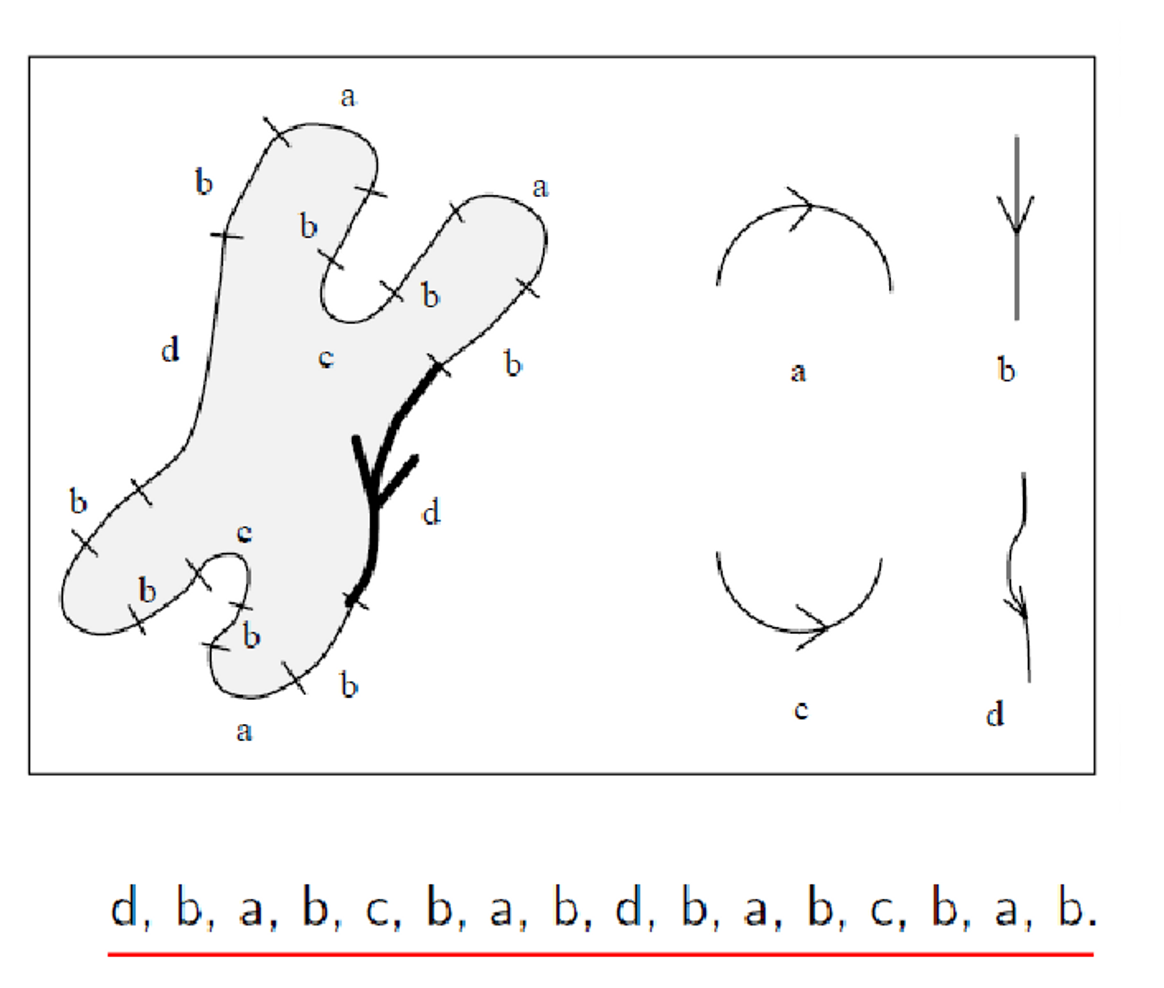
\includegraphics[scale = 0.3]{images/chain_codes.png}
\end{figure}
\subsubsection{geometrický popis}
přímost hranice - poměr mezi celkovým počtem bodů hranice a počtem bodů, ve kterých hranice mění směr\\
\begin{figure}[H]
    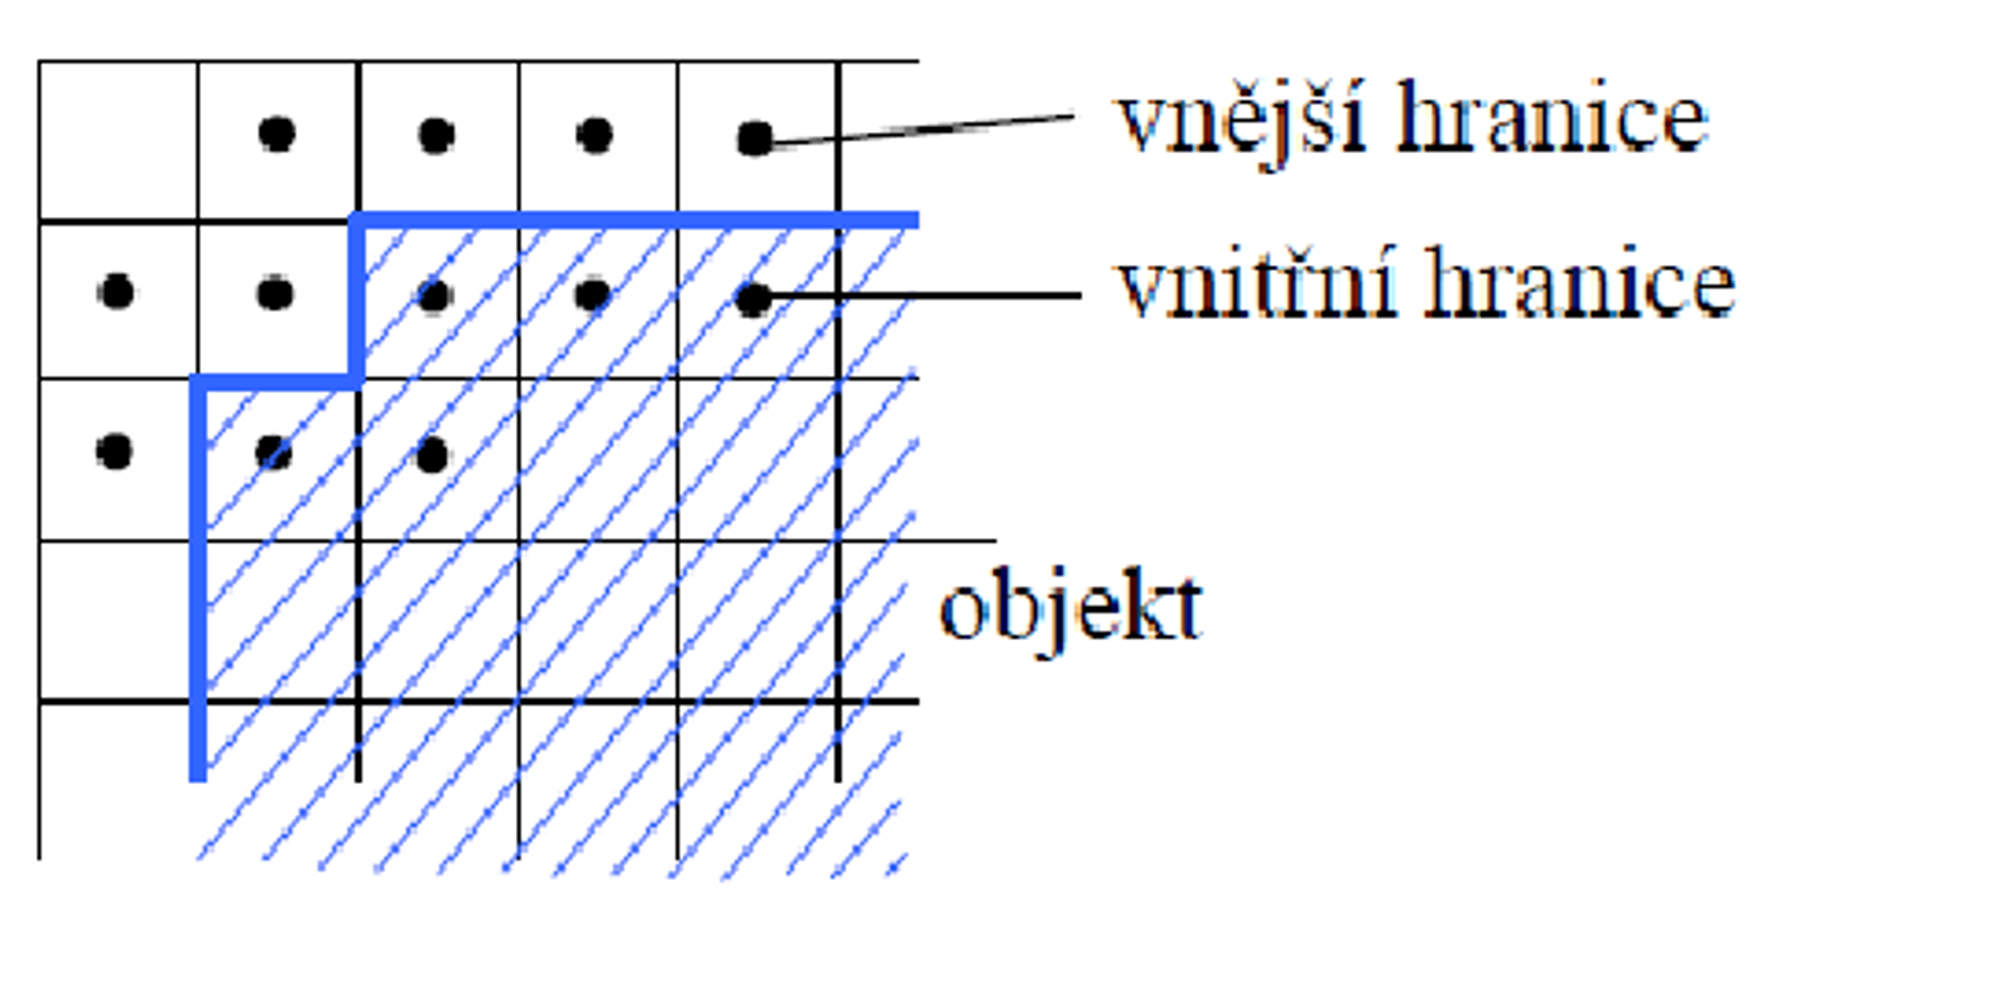
\includegraphics[scale = 0.2]{images/geometricky_popis.png}
\end{figure}
\newpage
\subsection{Klasifikace}
rozpoznávání předmětů spočívá v jejich zařazování do tříd - klasifikátor\\
Metody rozpoznání:
\begin{itemize}
    \item statické příznakové - zaměřují se na měřitelné veličiny objektu
    \item strukturní syntaktické - identifikace elementů objektu a analýza vztahů mezi nimi
    \item hybridní
\end{itemize}
(jsou i další, toto jsou ty hlavní)\\
\subsubsection{Učení}
\begin{enumerate}
    \item volba formálního popisu
    \item návrh rozhodovacího pravidla klasifikátoru
    \item způsob učení klasifikátoru - s učitelem, bez učitele
\end{enumerate}
\subsubsection{Příznakově popsané předměty}
obraz je sloupcový vektor, jehož souřadnice tvoří vektory\\
jednotlivým třídám odpovídají shluky obrazů, které lze oddělit vhodnou křivkou pomocí diskriminačních funkcí

\begin{figure}[H]
    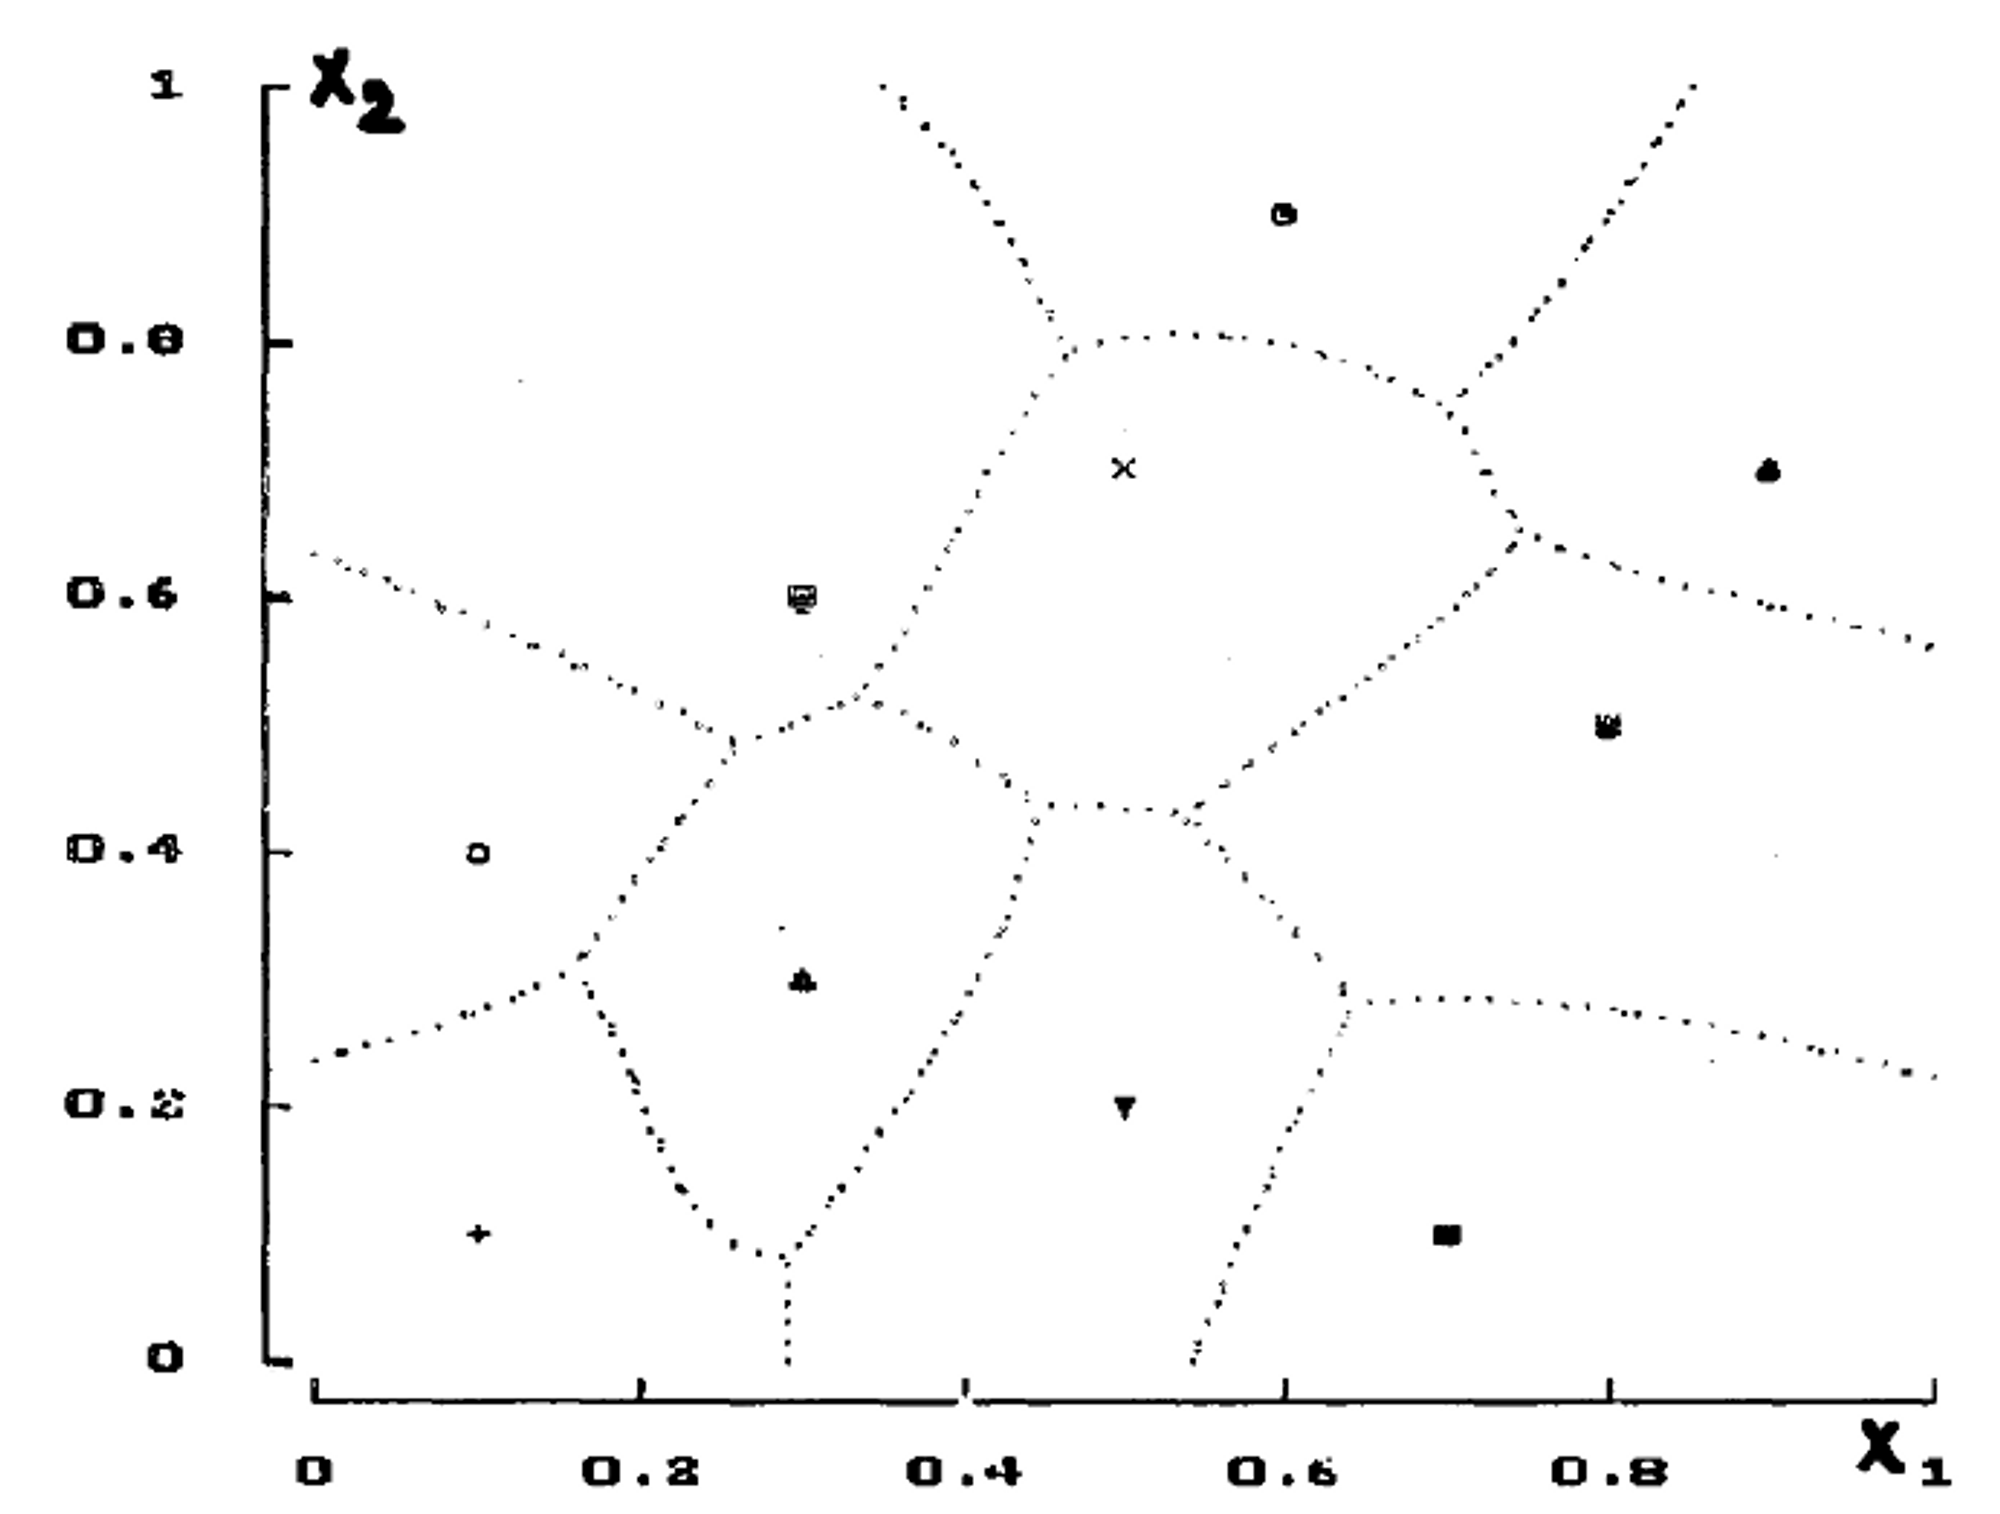
\includegraphics[scale = 0.2]{images/priznakove.png}
\end{figure}

\subsubsection{Syntakticky popsané předměty}

Identifikace elementů objektu a analýza mezi nimi\\
Vužívá primitiva což jsou informace o struktuře nebo kvantitativních či kvalitativních vlastnostech předmětu.\\
Vztahy mezi primitivy se nazývají relace.\\
Klasifikace vychází z teorie formálních jazyků.\\
Primitivum je popsané terminálem, množina terminálů se nazývá abeceda. Řetěz terminálovů pak tvoří větu. Věty popisují objekty, které patří do třídy daného jazyka.\\
Rozhoduje se zda věta popisující objekt patří či nepatří do do některé třídy.\\
\begin{figure}[H]
    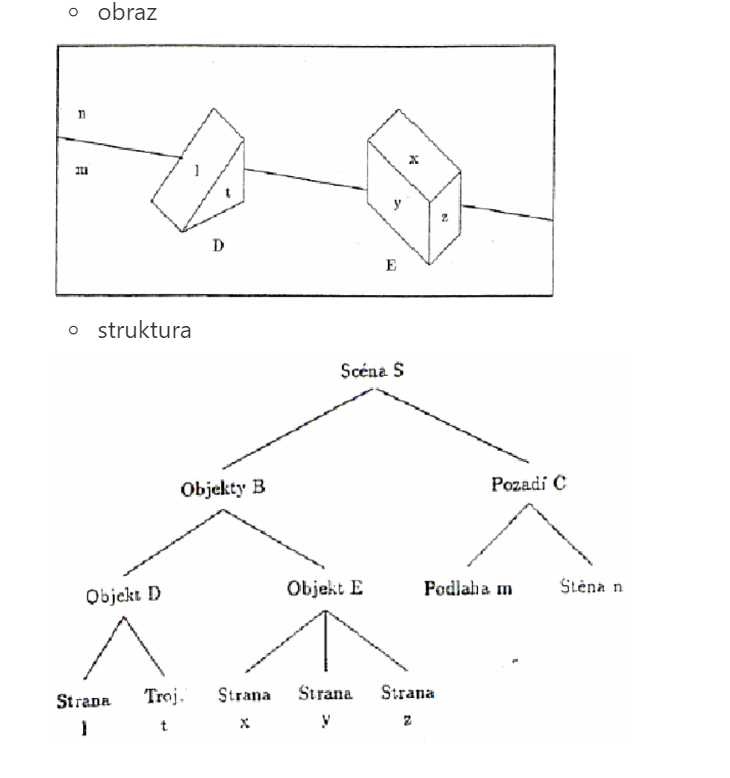
\includegraphics[scale = 0.7]{images/syntakticke.png}
\end{figure}
